%!TEX root = ../PhDThesis.tex



% *********************************************************************************************************************
\chapter{Studying caf\'{e} talk around smartphone-based VUI use}\label{ch:empirical cafe}
% *********************************************************************************************************************



\begin{revisedsubmission}[JR-2a: Refocus analysis onto the members problems being addressed with technology use]
This chapter presents the study of friends socialising face-to-face as a group in a neighbourhood caf\'{e}, and examines their interactions around the use of the `natural language' \acfp{VUI} on their personal mobile devices.
The previous work in \autoref{ch:empirical pub} explored how conversation in a pub unfolded with and around the use of the \acfp{GUI} on mobile devices, and how these device-based interactions were interleaved within the conversation amongst groups of friends.
This analysis revealed some pragmatics of how cooperative interaction occurred in, through, and around the use of the mobile device.

The work in this chapter pivots to considering how conversation unfolds around the use of a newer innovation, the `personal assistant' on mobile devices, which is interacted with primarily as a \ac{VUI} in combination with a \ac{GUI}.
It was previously posited in the outlook of the prior chapter that \acp{VUI} might lend themselves to collaborative interactions amongst the co-interlocutors around the device use due to the use of talk over touchscreen interactions.
This turned upon the notion that talk to \acp{VUI} would make the specifics of members' use of devices hearable to those around the device use.
\end{revisedsubmission}

The research in this chapter was previously published and presented at the Computer-Supported Cooperative Work \& Social Computing conference\footnote{See \citet{Porcheron2017}.}---a number of changes have been made \iresubmission*[JR-3c: Refocus the analysis on to the interactional accomplishments of members in the setting]{to address the research questions of this thesis}.

%since the presentation to address limitations in the work and to address problematic terminology highlighted from the questions.
%These changes are identified in \appref{app:changes-cafe} along with commentary on the change.
%Furthermore, a number of changes have been made to refocus the paper onto the collaborative efforts of members in the setting.



% *********************************************************************************************************************



\section{Introduction}\label{sec:empirical cafe introduction}
\begin{revisedsubmission}[JR-2a: Refocus analysis onto the members' problems being addressed with technology use]
Previously, this thesis studied groups of friends socialising in a casual-social setting---a pub---and explicated how members unproblematically interleave the use of touchscreen-based device interactions in talk to address problems at hand.
In accordance with this thesis' aim to explore the broader uses of technology use and its interwoven nature in casual-social settings, this chapter progresses to studying interactions that unfold around the use of voice-based `personal assistants' on devices.
To recapitulate, this type of space provides a suitable natural environment to observe participant behaviours with mobile devices ``in the wild'' in a perspicuous setting~\citep{Crabtree2006}.
A casual-social setting forms an environment in which individuals and groups can socialise with each other, that may be in or outside of the home or workplace, and that provides a level of comfort and relaxation for those who gather there.
In much the same way that a pub was previously regarded as a perspicuous setting for studying interactions around mobile device use, a caf\'{e} so too becomes such a setting for examination of naturally occurring interactions around device use.
Turkle succinctly emphasises this notion of communal spaces where we are together with others, but where mobile devices are present and in use:
\begin{quote}
    In this new regime, a train station (like an airport, a caf\'{e}, or a park) is no longer a communal space but a place of social collection: people come together but do not speak to each other. Each is tethered to a mobile device and to the people and places to which that device serves as a portal.
    \quoteauthor{\citet[p. 155]{Turkle2011}}
\end{quote}
The previous chapter explored how members of the casual-social setting account for and interleave device use within conversation, e.g. by bringing it up in conversation or sharing visibility of the screen.
This thesis posits that by shifting the input to the device to talk, away from interactions using a touchscreen, members may simultaneously and naturally account for the device interaction as an accomplishment of using the \ac{VUI}, given how talk is the most obvious form of making one's actions accountable:
\begin{quote}
    Talk is the most obvious and pervasive way in which members conduct their work and make whatever it is that they are doing into an intersubjectively recognisable and naturally accountable activity.
    \quoteauthor{\citet[p. 44]{Crabtree2012}}%[p. 44]
\end{quote}
Therefore, this study deviates from the prior examination of touch\-screen-based device use by \textit{requesting} participants to use the \ac{VUI} instead of the touchscreen preferentially.
Given this, it was decided to observe and record interactions in this successive study in a caf\'{e} due to lower background noises, although caf\'{e}s remain true to the established definition of a casual-social setting: they are places where groups of friends can gather to socialise and relax with each other.
As the work in this thesis is concerned not with device use as study of the technology, but rather with the study of interaction amongst multiple members of the setting while technology is being used during, asking participants to use the \ac{VUI} does not influence the outcome of the study.
Indeed, the focus is of the \textit{naturally occurring} interactions \textit{around} the device use.
\end{revisedsubmission}

As the name suggests, these \acp{VUI} are interacted with primarily through the user speaking, with software running on the device `recognising' the words spoken, and attempting to run the command or request made by the user.
Typically \acp{VUI} on personal mobile devices `listen' to the user and display the `understood' words as well as the course of action being taken by the device, or an error message.
In this sense, a \ac{VUI} on a portable device presents a composite, or \textit{hybrid}, of both \acp{VUI} and \acp{GUI}, in which users must provide commands or instructions through talking to a device without \textit{a priori} display of possible options.
In turn, users are presented with a \ac{GUI} to accomplish and understand the processing of their voice and the action taken by the device.

\begin{revisedsubmission}[JR-2b: Include further detail on the specific technology to understand its use in a public setting]
From a technical perspective, a factor behind the introduction of \acp{VUI} is that talk remains a flexible and pervasive method members routinely employ to accomplish a task\footnote{Beyond, of course, mere reasons of selling more products.}, i.e. the scope and capability to communicate through talk is much greater than that through a pre-designed touch-based \ac{GUI}, especially on small-screen devices given the potentially limitless use of vocabulary within human language.
Marketing materials from companies such as Apple Inc. have promoted their respective \acp{VUI} as allowing users to `get things done' with ease, allowing the user to talk to them as they would `to a friend'.
Moreover, research into talking with computers is long-stand\-ing, with work as far back as \citet{Licklider1960} remarking that ``there is a continuing interest in the idea of talking with computing machines''~\citep[p. 10]{Licklider1960}.
More recent work has pursued the ideas of talking machines (i.e. conversational agents) that act as companions for the elderly~\citep{Vardoulakis2012}, or virtual museum guides~\citep{Kopp2005}.
This thesis, however, is primarily concerned with another form of conversational agent---the `virtual butler' that helps people `get things done'~\citep{Payr2013}.
In particular, the study in this chapter will explore the practical use of the virtual butlers readily found on peoples' personal smartphones and tablets to make sense of just how these `butlers' are practically used in interaction to `get things done'.

While there are a plethora of commercial products as well as active research projects examining various aspects of creating and enhancing \ac{VUI} design, existing systems come with their own restrictions in terms of capability in translating spoken words and sounds into text, in parsing the text into machine understandable commands, and performing the desired actions with the understood commands.
These technical limitations are not the focus of this thesis but remain a factor in considering how members attend to and accomplish their interactional projects with the devices.
\end{revisedsubmission}

The marketing materials for these \acp{VUI}, marketed as \acfp{IPA}, suggest that they can be interacted with like any person might, and can respond to natural human talk. %\footnote{This further has the benefit of avoiding the use of two conflating initialisms: Conversation(al) Agent(s) and Conversation Analysis.}.
For example, two such systems, Siri (Apple Inc.) and Cortana (Microsoft Corporation), both appear to exude humour in response to general `conversational' input, questions, and instructions.
In turn, their responses to the user might be seen as sarcastic or entertaining.
\iresubmission*[JR-3a: Refocus the analysis as a video-supported ethnography]{While \acp{VUI} may provide the veneer of conversational intelligence, this study examines the interactional accomplishment of using a \ac{VUI} in and through interaction, grounded in the empirical evidence derived from a video-supported ethnography, and reveals the cooperative nature of interaction in, through, and around the use of the device.}
%The notion of conversational nature of these \acp{VUI} is later returned to in reflection in \autoref{}

On a large proportion of current mobile devices, the \ac{VUI} may be triggered through one of two means: by pressing a physical or on-screen button, or by the utterance of a `hotword' that enables the interface (e.g. ``Hey, Siri'').
The human interlocutor (i.e. the user) then talks to the assistant, and is able to engage in dialogue and ask questions (e.g. about the weather), or give instructions (e.g. to call someone); the \ac{VUI} responds either by speaking back or by displaying a response on the device's screen.
In essence, the assistant is a natural language interface to the device's existing functionality.
\autoref{fig:empirical cafe introduction screenshots} presents three screenshots of the most popular commercial \acp{VUI} on smartphones\footnote{This is anecdotal based on smartphone ownership numbers.} responding to different types of questions.
As shown in the dialogue with Siri, responses may contain humour in addition to factualness.
Furthermore, in addition to task-oriented questions and instructions, some commercially available \acp{VUI} also respond to general questions such as ``how are you?'' and ``what's your favourite colour?'', further anthropomorphising the assistant.

\begin{figure}[bth]
    \subfloat[Siri]
    {\label{fig:empirical cafe introduction screenshots siri}%
    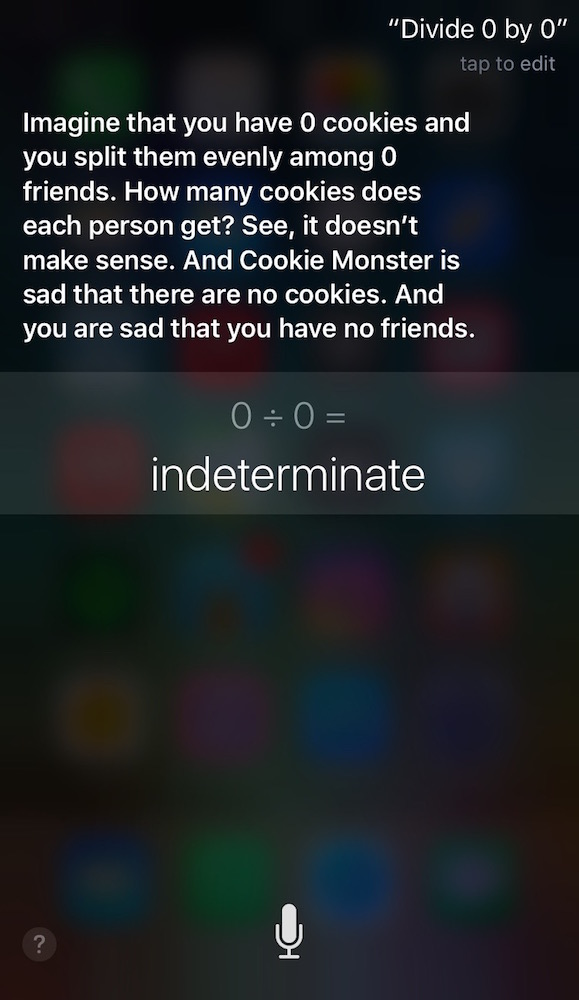
\includegraphics[width=.3\linewidth]{Graphics/3-2-Empirical-Cafe/ScreenshotSiri-Redacted}} \quad
    \subfloat[Google Now]
    {\label{fig:empirical cafe introduction screenshots googlenow}%
    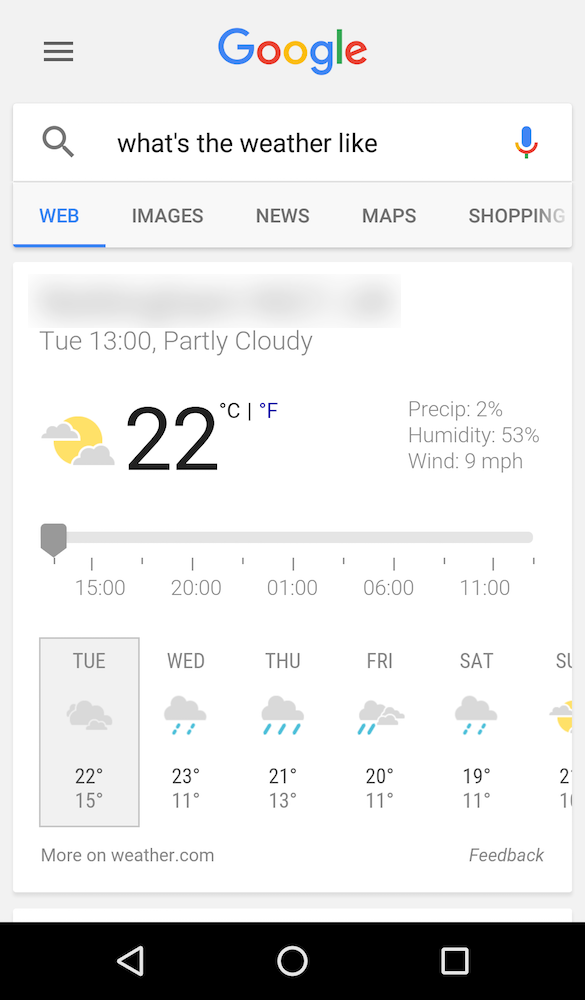
\includegraphics[width=.3\linewidth]{Graphics/3-2-Empirical-Cafe/ScreenshotGoogleNow-Redacted}} \quad
    \subfloat[Cortana]
    {\label{fig:empirical cafe introduction screenshots cortana}%
    
\includegraphics[width=.3\linewidth]{Graphics/3-2-Empirical-Cafe/ScreenshotCortana}}
    \caption[Example screenshots of different `Intelligent Personal Assistants' on commercially-available smartphones]{Example screenshots of different `Intelligent Personal Assistants' on commercially-available smartphones. The screenshots of Siri, Google Now, and Cortana are copyright Apple Inc., Google Inc., and Microsoft Corporation respectively. These screenshots were taken in 2016.}\label{fig:empirical cafe introduction screenshots}
\end{figure}

Early iterations of \acp{VUI} were focused on single tasks, such as \citet{Zue2000}'s JUPITER that was capable of providing weather information.
This particular system, as with others at the time, relied on people making telephone calls to interact with it, with the system engaging in dialogue with the interlocutor by talking back in a `conversational' manner.
As network connectivity and accuracy with automatic speech recognition improved, \acp{VUI}, such as InCa~\citep{Kadous2004}, were able to operate on portable mobile devices by making use of remote computing power and wireless communication technologies.
\acp{VUI} are now readily found on many devices such as smartphones, tablets, watches, and even televisions.
Additionally, although such systems fail to mimic human talk fully, \citet{Pelikan2016} were able to reveal the succinctness of how people adapt their talk to an assistant's needs and capabilities, making their interactions more successful.
Their work focused on a dyadic face-to-face conversation with a humanoid robot and was able to reveal a number of difficulties individuals face in such talk.
In this work, there is a pivot to considering how this talk unfolds as a situated action within a multi-party conversation.
A number of pieces of work focused on \acp{VUI} have suggested a number of positive aspects in order to justify their development further.
In one case, \citet{Jones2014} describe how a voice-controlled personal assistant could be used to support collaboration amongst those gathered around an interactive smart table, or for use in hands-free or `eyes-free' interaction while driving a car~\citep{Cycil2013}.
Others such as \citet{Luger2016}, however, paint a more challenging picture.
Through interviews, they found that there still exists a ``gulf between user expectation and experience''~\citep[p. 1]{Luger2016} with existing conversational agents and user expectations.
This gulf stems from people's perceptions that such systems should deliver more than they presently do and for issues with the \ac{VUI} communicating system functionality.
Innovations to address this gulf include features such as displaying understood text on a screen, voice typing~\citep{Kumar2012a} (i.e. live dictation), and the grounding (i.e. affirmation) of spoken input through responses~\citep{Clark1991,McTear2016}, although peoples' reported experiences suggest that numerous problems still remain.
By exploring the interactional accomplishment of using \acp{VUI} on smartphone devices \textit{in vivo} within a social gathering, and by employing a conversation analytic approach, a rich description of the collaborative work performed by members that occurs in, through, and around the \ac{VUI} use can thus be explicated.



% *********************************************************************************************************************



% \section{Research questions}\label{sec:empirical cafe rqs}
% The work in \autoref{ch:empirical pub} explored the collaborative practices that occurred within a social gathering in a pub while members made use of mobile devices through the touchscreen only, and in \ref{sec:empirical pub discussion coop} the practicalities of how members methodically collaborated in and through mobile device use was discussed.
% These primarily drew upon articulation work and accounting practices that members did to continue to display social engagement while embedding the device use within the social interaction.
% One potentially interactionally problematic feature of these sequences was the need for members to engage in accounting for device use because interacting with a (relatively) small personal device such as a smartphone precludes others from an awareness of device interaction that is unfolding.
% It was posited, and so is studied in this chapter, that speech interaction with a mobile device could free members from this practice as the production of talk is naturally accountable and so diminishes the necessity for members to methodically account for the use as a separate sequential act (see \ref{sec:empirical pub discussion problematic}).
% This chapter, then, sets out to unpack the work of using speech as part of the device interaction with the smartphone, and will continue to reveal the details of how interaction with the device is routinely embedded within conversation (RQ1), and how members engage in collaborative action in and through the interaction with the device (RQ2):
% \PrintRQ{1}
% \PrintRQ{2}



% *********************************************************************************************************************



\section{Study design}\label{sec:empirical cafe design}
 \begin{revisedsubmission}[JR-3a: Change EMCA to `study informed by EM']
A brief description of the setting in which the observations were undertaken is provided below, including details about the participants, and also the rationale for continuing to adopt an ethnomethodological and analytic orientation.
The study was approved by the university's School of Computer Science Research Ethics Committee.
\end{revisedsubmission}



% *********************************************************************************************************************



\subsection{The caf\'{e} as a study setting}\label{sec:empirical cafe design setting}
\begin{revisedsubmission}[JR-2b: Include details on the selection of the setting and the perspicuousness of the setting to the activity under study]
This chapter extends the work begun in the study of pub talk around touchscreen-based device use in the prior chapter by pivoting to exploring talk in a caf\'{e} around smartphone-based \ac{VUI} use.
In order to situate the study, a casual-social setting was chosen (see \ref{sec:empirical pub design setting}) to conduct a number of observations of friends socialising together.
As discussed, this study deviates from the prior examination of touchscreen-based device use by \textit{requesting} participants to use the voice-based personal assistant on their device instead of typing.
All participants were required to have used the assistant before the study.
It was supposed that given the identical premise of participant activity (i.e. of a gathering to socialise and relax), that the difference in setting would not be influential on the participants' use of devices (nevertheless, such a concern was not a primacy in this research given the analytic orientation, as discussed in the next section).

Although the particulars of activities that take place in a caf\'{e} may differ from that of a pub, to those who choose to gather there as a group of friends, the purposes remain the same: to socialise and relax together.
In other words, although the food may be different and there may be less sport or alcohol, the purposes for being in the setting as a group remain consistent.
Indeed, caf\'{e}s were also included within the definition of ``third places''~\citep{Oldenburg1989}, from which this thesis' more encompassing definition of a casual-social setting was formed.
Oldenburg defined third places as spaces that are outside the home or work environment that support gathering, socialising, and relaxation for groups and individuals, and with this definition, a caf\'{e} is the epitome of a such a setting.
Work that has studied interaction in caf\'{e}s remarks upon how they provide a ``common code of conduct''~\citep[p. 210]{Laurier2001}  that is both informal yet still provides a guidance of behaviour that is adhered to by members, but typically lack ``complex articulation and coordination work'' found in more formal settings~\citep[p. 222]{Laurier2001}.
Laurier, a number of years later, in studying interactions in a caf\'{e}, introduces caf\'{e}s in the UK and USA as ``familiar nodes in the network of gathering places that remain a necessity for the accidental tourists, be they business executives, chefs or mathematicians, who shuttle back and forth stitching regions together''~\citep[p. 5]{Laurier2008a}.
It is through this text that the significance of caf\'{e}s is realised as spaces in which different people in different situations gather for various purposes.
Indeed, during the observations that took place for the work in this thesis, the caf\'{e} received a constant stream of visitors, some merely taking drinks to go, and some meeting up with others, some brought children and some arrived as groups of friends.
Therefore, such a setting is perspicuous to observe a gathering of friends socialising.
\end{revisedsubmission}



% *********************************************************************************************************************



\subsection{Collecting data in the caf\'{e}}\label{sec:empirical cafe design participants}
In the study, a neighbourhood caf\'{e} was selected that served hot and cold food, cakes, and drinks.
The caf\'{e} is in a residential suburb of Nottingham, within a pavilion at a local park and nearby to schools and a university.
Suitable times for observations were agreed between the caf\'{e} and participants, allowing for video and audio recording of the friends talking during a gathering lasting up to ninety minutes.
All sessions were recorded on weekday afternoons when the caf\'{e} was open to the public.
\iresubmission*[ER-F, ER-G1: Specify how data were collected in practice]{Video capture was completed by two fixed wide-angle cameras on tripods with an audio recorder placed on the table to allow for clearer capture of talk between the participants.}

Groups of friends were recruited via email and social media to visit the caf\'{e} together for the purposes of socialising.
Prior to the study, participants were asked whether they had previously used a personal assistant on their mobile device, although there was no frequency or expertise required by them in order to take part.
Three groups of four friends were recruited to go to the caf\'{e} together over a two-month period.
Seven participants self-identified as male, and five as female; they ranged in aged from 22 to 37. % (M = 28.75).
All participants gave informed consent and were reimbursed for their time with a shopping voucher.
During the studies, all participants drank various drinks, some ate cake, and one brought some light reading with them to do as they were chatting with their friends.



% *********************************************************************************************************************


%\subsection{Methodology}\label{sec:empirical cafe design methodology}
The study approach is most aptly described as participant-observer, with a researcher present at the table conversing with the group where relevant.
The group of friends met the researcher at the caf\'{e} and were asked to complete a consent form prior to data capture.
They were free to move about in the caf\'{e} although primarily sat around a single table as they socialised, drank, and ate cake with each other.
For the study, participants were asked to preferably use the personal assistant on their mobile devices instead of typing where possible\footnote{The information sheet provided to participants prior to the study is included in \appref{app:studyinfo-cafe infoconsent}} adjusting the study to be as close to `natural' as feasibly possible to that of a study of interactions that are somewhat prescribed by very nature of the enquiry.
However, the methodological approach to studying interaction remains steadfast given the analytic orientation to the accomplishment of members in and through interaction, irrespective of \textit{reasons why}.

As per \autoref{ch:empirical pub}, there was no requirement to use a device, and there were no tasks set for the friends to perform during the study.
The idea of curating a number of tasks for groups to perform with \acp{VUI} during the sessions was considered, however following a pilot study in which participants were given `free reign' on what activities to perform during the study, and told to converse as they normally would, it was concluded that this was not needed–--people still chose to use the \acp{VUI} on their devices.
Therefore, participants were simply asked that they socialise and when the opportunity arose, they use a \ac{VUI} instead of typing, if appropriate.
After the study, a number of informal questions to gauge feedback and gather personal perspectives on the use of \acp{VUI} were asked.
However, this group interview was used as a debriefing exercise rather than to shape the findings.



% *********************************************************************************************************************



\subsection{Analysing the collected data}\label{sec:empirical cafe design analysis}
\begin{revisedsubmission}[ER-G1: Add further information about the analysis of the corpus, primarily the selection of fragments]
To analyse the collected corpus, as with the prior study, an analysis shaped by ethnomethodology~\citep{Garfinkel1967, Sacks1974} was performed.
Through this, the orderly and situated practice of using \acp{VUI} in conversation was explicated.
This analysis required the watching of the collected corpus multiple times, in order to segment and identify relevant fragments of data consisting of \ac{VUI} use.
Firstly, fragments were watched (and re-watched), with the methodical actions of members within the setting catalogued and indexed to identify instances where a mobile device and a \ac{VUI} was used.
Timestamps and descriptive language were used to construct a record of the interactions that took place, which allowed for iterative re-examining of prior data with relative ease to help gain an overall impression of the data collected across all the sessions.

Three fragments were selected for presentation in this chapter.
In line with best practice, as summarised by \citet{Heath2010}, each fragment progressively reveals the organisation of interaction with and around the use of the device:
\begin{quote}
    As you build an argument the analysis should be progressively revealed and emerge by virtue of the presentation of each successive extract. Furthermore the fragments should become more delicate and complex such that the audience can learn how to see the phenomena and can follow the argument as it unfolds.
    \quoteauthor{\citet[p. 111]{Heath2010}}
\end{quote}
In the three fragments to be presented, the first illustrates a typical use of a \ac{VUI} on a smartphone to introduce new information to the conversation that will set the scene for the interactions that unfold.
The second fragment introduces a more complex case that reveals how users perform additional actions to get the \ac{VUI} to work as desired.
The final fragment introduces an interactionally problematic case where a member uses the \ac{VUI} to establish its capability, revealing the richness and complexity of interaction around the use of a \ac{VUI} in a caf\'{e}.

The work was oriented to unpacking the retrospective-prospective character (see \ref{sec:background approach em sequentiality}, \citet[pp. 35--75]{Garfinkel1967}) of members accomplishing the work of using a \ac{VUI} in this setting, in and through their ongoing social interaction.
This orientation necessitated the identification of interactional accomplishments that occasioned the use of the \ac{VUI}.
This included how the device was introduced, the instruction or question that formed the request to the \ac{VUI}, the actions (in-talk and physical movements) of members in the setting throughout the activity, and so on.
In other words, this orientation, and the resulting analysis, allowed for the formation of a comprehensive understanding of the activities performed by members in using the \ac{VUI}.%, as per RQ1.
%In turn, the collaborative efforts undertaken by members in the setting were revealed through the sequences of contingent and contextually shaped action, as per RQ2.
\end{revisedsubmission}

In total, 40 episodes of \ac{VUI} use in the sessions were identified (some of which were overlapping), with episodes ranging from a few seconds to a nearly five minutes in length.
\iresubmission*[ER-G1: Add further information about the analysis of the corpus, primarily the selection of fragments]{A substantive review of the episodes was performed to examine the interaction that unfolded, honing in on episodes that represented observable-reportable intersections of the use of the \ac{VUI} and conversation for a more in-depth analysis.
Six fragments were then transcribed with both verbal (i.e. talk) and non-verbal actions (e.g. gestures and other interactional resources) being carefully noted.
These fragments were selected in line with the aims of this research to reveal the social organisation of device use in the use of \acp{VUI} in and through conversation and that were deemed to warrant further investigation.%, with each fragment being reviewed individually and discussed collaboratively with other researchers multiple times.
}



% *********************************************************************************************************************



\section{Findings}\label{sec:empirical cafe findings}
\begin{revisedsubmission}[JR-3a, JR-3c: New structure and framing of the analysis]
Data from the fieldwork will now be introduced and presented over a series of `data excerpts'---these excerpts form fragments that \textit{vividly exhibit}~\citep{Crabtree2012} the actions of members within the collected corpus.
Each of these fragments exhibits the activities of members' observed practices of how members made use of the \acp{VUI} on their personal devices in the caf\'{e}.
% The first fragment provides a preliminary sense of what interaction with a \ac{VUI} \textit{looks like}, revealing how devices can be used to retrieve new information for conversation (c.f. \ref{sec:empirical pub findings newinfo}).
% The second fragment introduces a more complex ample of how members answer questions in conversation using the device, and how collaborative efforts ensure in getting a device to work.
% The third fragment introduces interaction that unfolds as a result of the design of \acp{VUI}---using the \ac{VUI} to establish its capability.
% Throughout the explication of the fragments, the practice of how device use is used as a mundane activity in ``caf\'{e
% } talk'' will be established.
\end{revisedsubmission}

%By orienting to the sequentiality of using \acp{VUI} on a portable device in conversation, the nature of how the members' actions were occasioned in and through interaction, and, sequentially, what this methodical and situated practice brought about are explicated.
%Vivid exhibits~\citep[p. 112]{Crabtree2012, Bannon1993} of the accomplishment of using \acp{VUI} are provided to exemplify the orderly practice of members and present a rich picture of how members' use of their mobile devices unfolds.
In total, the corpus consists of 123 utterances to \acp{VUI} by members, across 40 distinct episodes of data from a corpus consisting of 3.6 hours of video data.
In particular, this chapter will reveal (1) how members perform a request with their device, (2) how members orient to and appropriately deal with the request and the \ac{VUI}'s response to the request, and (3) how members collaborate through the interaction with the \ac{VUI}. 

\appref{app:notation} provides details of the transcript notation used in this thesis.
All names and identifiable information within the transcripts provided are entirely fictional.

\begin{revisedsubmission}[JR-3a, JR-3c: Introduce the new fragments structuring]
%ata from three distinct fragments are now presented with the following corresponding findings: the first fragment  revolves around where a member of the setting uses the \ac{VUI} to \textit{introduce new information for conversation} (akin to what was identified previously in \ref{sec:empirical pub findings newinfo}, see \ref{sec:empirical cafe findings newinfo}),  the second focuses further on people using a \ac{VUI} to answer a question to verify information in conversation (see \ref{sec:empirical cafe findings answering}), and the final fragment introduces a situation in which individuals work to identify and confirm the capability of a \ac{VUI} (see \ref{sec:empirical cafe findings capability}).

% In the following fragments, The use of a \ac{VUI} will be shown to consist of two key instrumental activities across all fragments of data in this chapter:
% \begin{itemize}
%     \item Preparing and addressing the \ac{VUI}, and
%     \item Responding to the \ac{VUI}
% \end{itemize}
\end{revisedsubmission}



% *********************************************************************************************************************



\subsection{Introducing new information for conversation}\label{sec:empirical cafe findings newinfo}
\begin{revisedsubmission}[JR-3a, JR-3c: This section is new, reconstructed from prior analysis]
The first fragment, called \textit{When Does the Sun Go Down?}\footnote{The complete fragment is included in \appref{app:fragments-cafe sunset}.}, that commences in \autoref{frag:empirical cafe findings newinfo-i}, consists of four friends: Arthur, Harry, Sally, Julia, and the researcher.
The friends are meeting late afternoon during winter and the sun is shining into Harry's eyes.
He holds his hands in front of his eyes although he refuses to move because he will \QF[01]{...be fine in like three minutes}.
The friends joke about this experience, and that this forms part of their study (lines 08–15), but this challenge of the blinding sunlight establishes the interactional project that ensues.
Later in the next excerpt, Julia uses her iPad, which she had out on the table already, to find the time of sunset as a result.

\begin{inlinefrag}
    {\fragresubmission{JR-3c, ER-H: Revised fragment that is shorter, with labels on the image for the speakers}
    \begin{transcript}
        \by HAR {i’ll be fine in like three minutes ((holds hands in front of} \\
        \by     {eyes))} \\
        \by RES {keeps coming back as well like} \\
        \by SAL {as soon as you cha\emph{nge} it comes back} \\
        \by JUL {yeah yeaha} \\
        \later  {0.3} \\
        \by RES {there’s actually just someone out there with a light!} \\
        \by ALL {((laugh))} \\
    \end{transcript}
    \caption{When Does the Sun Go Down? (i)}\label{frag:empirical cafe findings newinfo-i}
    \begin{figure}[bth]
        \centering
            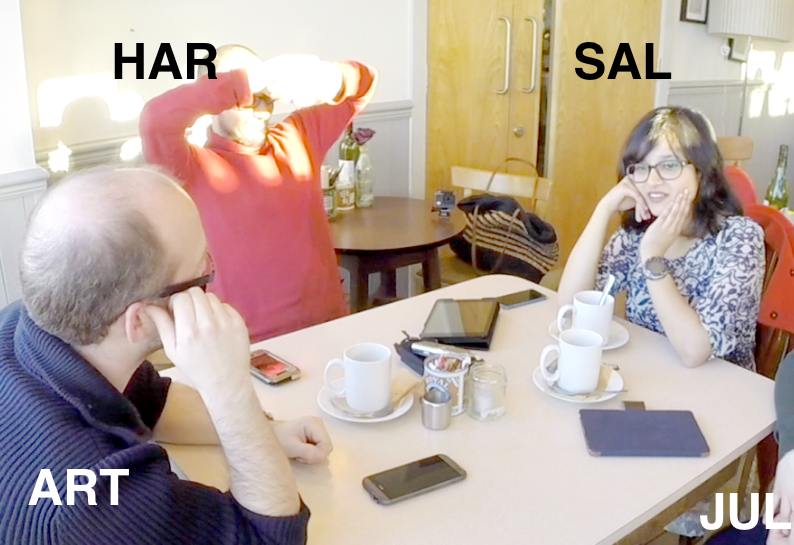
\includegraphics[width=.7\linewidth]{Graphics/3-2-Empirical-Cafe/FragmentSunset-1}%
        \caption{HAR blocks the sunlight in his eyes (\autoref{frag:empirical cafe findings newinfo-i}: When Does the Sun Go Down? (i), line 1)}\label{fig:empirical cafe findings newinfo-i}
    \end{figure}
    }
\end{inlinefrag}

In this opening excerpt, the group jokes about the sun shining through a nearby window into Harry's eyes as a result of the time of day (approximately evening time, around sunset).
This occasions, as will become evident in the following excerpts, Julia to use her \ac{VUI} to retrieve the time of \textit{sunset} for this given location.
This work to establish the time of sunset addresses the ongoing concern established in conversation about the sun in Harry's eyes, and responds to his remark that he will \QF[01]{be fine in like three minutes}, with the use of the \ac{VUI} commenced by Julia to introduce new information to \textit{verify} his claim. The next two sections, centred around two excerpts that follow Julia as she seeks new information for the conversation:
\begin{enumerate}[label=(\roman*)]
    \item \nameref{sec:empirical cafe findings newinfo addressing}, and
    \item \nameref{sec:empirical cafe findings newinfo collab}.
\end{enumerate}

As will be evident through the sequential revelation of members' actions, the \ac{VUI} will be introduced and used with the address of a question occasioned in and through the conversation.
The nature of multi-party conversation and making a device interaction accountable will allow members to engage with the interaction at hand in the completion of one member's interactional project to verify the time of sunset.
\end{revisedsubmission}



% *********************************************************************************************************************



\crpagebreak\subsubsection{Addressing the question to the VUI}\label{sec:empirical cafe findings newinfo addressing}
\begin{revisedsubmission}
The discussion continues before the next excerpt, \autoref{frag:empirical cafe findings newinfo-ii}, picks up the conversation.%, with the members of the group joking that the light in Harry's eyes is a result of someone standing outside the window with a torch, or as a result of the study itself.

\begin{inlinefrag}
    {\fragresubmission{JR-3c, ER-H: Revised fragment that is shorter, with labels on the image for the speakers}
    \begin{transcript}[16]
        \by JUL {[ ((removes cover from device but leaves open)) ]} \\
        \by SAL {((laughs))} \\
        \by JUL {((presses button on device))} \\
        \by HAR {there we go!} \\
        \by JUL {\textbf{what’s the time of sunset?}} \\
        \later  {1.3} \\
        \by ALL {((gaze at the tablet))} \\
        \later  {3.0} \\
        \by JUL {ok! \textit{// ((device displays clock)) //}} \\
        \by ART {((leans in to look))} \\
        \by SAL {that’s [ a~~~~~~] fucking analogue clock it pisses me off!} \\
        \by HAR {~~~~~~~[ today? ]} \\
        \by HAR {ilunno (0.6) 24 hour=} \\
        \by JUL {<no no no!> it misunderstood actually (0.8) understood what’s the} \\
        \by     {~[ time ]} \\
        \by HAR {~[ time ] now} \\
    \end{transcript}
    \caption{When Does the Sun Go Down? (ii)}\label{frag:empirical cafe findings newinfo-ii}
    \begin{figure}[bth]
        \centering
            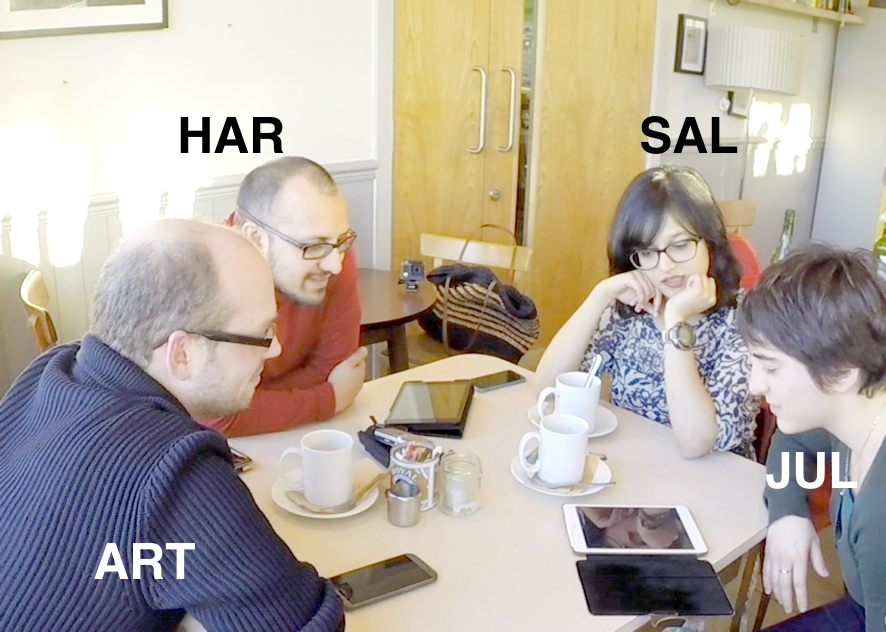
\includegraphics[width=.7\linewidth]{Graphics/3-2-Empirical-Cafe/FragmentSunset-2}%
        \caption{All members gaze at the tablet (\autoref{frag:empirical cafe findings newinfo-ii}: When Does the Sun Go Down? (ii), line 25)}\label{fig:empirical cafe findings newinfo-ii}
    \end{figure}
    }
\end{inlinefrag}

First, this excerpt is unpacked.
As the laughter begins to die down within the group at the start of the excerpt, Julia removes the cover from her device, which she has on the table (line 16); she waits for the group laughter to die down, presses the home button (line 18), and begins her utterance as Harry finishes remarking that the sun has now moved (line 19).
Julia uses her device's \ac{VUI} to ask for \QF[19]{the time of sunset}.
As she does this, she fixes her gaze at the screen, which displays a loading animation while the device is awaiting input.
At this point, all members lean in towards the device, as shown in the image, and demonstrate an awareness of an impending response from the \ac{VUI}.
As she began her request, Harry utters \QF[18]{there we go} in direct response to the sun no longer coming through the window directly into his eyes (inferred by his shift in posture, including no longer covering his eyes with his hands).
Nevertheless, Julia pressed ahead with the question, having begun the performance of preparing the device for the address by pressing the button.

After a few moments, the \ac{VUI} returns the time for the local area as an analogue clock.
A number of comments on this are passed: Sally comments on the presentation of the time (line 26) and Harry questions if that is for the present day (line 27).
Julia then interrupts the talk and retorts that she has realised the device has \QF[29]{misunderstood actually} and that the \ac{VUI} is presenting the current time, not the time of sunset.

By explicating the distinct sequential actions taken by members as the device is used, the ways in which members practically reason about how a \ac{VUI} responds to a request and attend to the \ac{VUI}'s response become evident (e.g. by leaning in, rotating gaze, not over-talking the \ac{VUI} or \ac{VUI}-user).
In this exhibit, Julia reasons about the failed outcome of the request to the \ac{VUI} through examining the displayed response, and makes this accountable to all (line 25) through her verbal report.
Her position and access to the device affords her greater visibility (as seen in the image in \autoref{fig:empirical cafe findings newinfo-ii}) of the response from the device, which typically displays the `transcribed' text of what the device `understood'.
Through her vocalised interpretation of the output of the \ac{VUI}, she provides an explanation for the problem source---or rather, starts to---as she realises it \QF[29]{understood what's the---} and Harry, who seemed to question the answer (line 27) completes her sentence with \QF[31]{time now}.
Harry's completion of Julia's utterance exemplifies that he is in accord with her reported interpretation of the source of technical trouble.

Through the ongoing interaction, as will be revealed in the next excerpt, members collaboratively reason that the response was not as expected and that this must be because the transcription of the request by the \ac{VUI} was wrong.
\end{revisedsubmission}



% *********************************************************************************************************************



\subsubsection{Collaboratively finding new information}\label{sec:empirical cafe findings newinfo collab}
\begin{revisedsubmission}
Julia's previous assessment that the device was showing the current time, as opposed to the time of sunset, (lines 30---32)  leads to a proposal to ask a different question (line 36) to the device from Julia.
In turn, the members collaboratively find words to return a successful result, as examined in this next excerpt, with Julia proposing a follow-up question, and Harry providing a suggestion of the wording she should use (line 35).

\begin{inlinefrag}
    {\fragresubmission{JR-3c, ER-H: Revised fragment that is shorter, with labels on the image for the speakers}
    \begin{transcript}[32]
        \by JUL {so-} \\
        \by ART {soaoah yeah\intUp} \\
        \by JUL {shall i ask (1.6) um:=} \\
        \by HAR {~~~~~~~~~~~~~~~~~~~~~=what time will the [ sun set? ]} \\
        \by JUL {~~~~~~~~~~~~~~~~~~~~~~~~~~~~~~~~~~~~~~~~~[ ((holds button)) ]} \\
        \by JUL {\textit{// ((audible chime)) //}} \\
        \later  {4.0} \\
        \by JUL {\textit{ // ((on screen text: go ahead i’m listening\ldots)) //}} \\
        \later  {0.3} \\
        \by JUL {\textbf{when does the sun go down?}} \\
        \later  {2.9} \\
        \by JUL {sunset will be at [ seventeen thirty two ]} \\
        \by ART {~~~~~~~~~~~~~~~~~~[ ther:::e you go~~~~~~]} \\
    \end{transcript}
    \caption{When Does the Sun Go Down? (iii)}\label{frag:empirical cafe findings newinfo-iii}
    % \begin{figure}[bth]
    %     \centering
    %     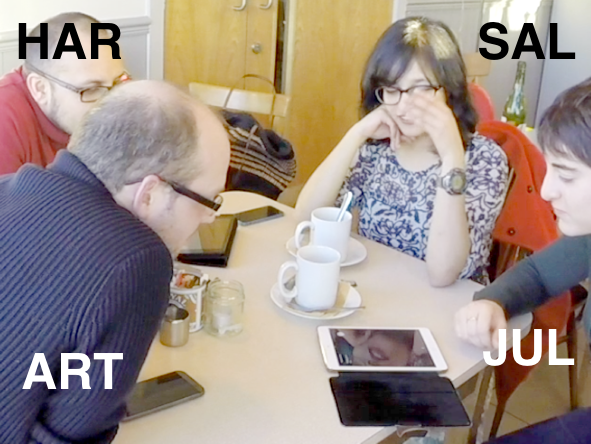
\includegraphics[width=.7\linewidth]{Graphics/3-2-Empirical-Cafe/FragmentSunset-3}%
    %     \label{fig:empirical cafe findings newinfo three}
    %     \caption{Members inspect the outcome of the request (\autoref{frag:empirical cafe findings newinfo-iii}: When Does the Sun Go Down? (iii), line 22)}\label{fig:empirical cafe findings newinfo-iii}
    % \end{figure}
    }
\end{inlinefrag}

In this final excerpt, Harry proposes a slightly different question (line 35) although ultimately Julia asks \QF[41]{when does the sun go down?}, to which the \ac{VUI} provides an accepted answer as revealed in Arthur's comment of \QF[44]{there you go}.
Although the time is visible on the screen and all members look at it, Julia also provides an audible report of the time displayed (emblematic of the \textit{hybrid} nature of \ac{VUI} interaction on a smartphone also making use of the screen).
This excerpt reveals how members can collaborate on a project by working together to use a device, exemplified in this fragment through the demonstrable reasoning of suggesting the cause of trouble and through reformulating the request by the members.
In the fragment, across the three excerpts, Julia interprets the initial result from the \ac{VUI} as incorrect (line 29), but then reasons about the response, reveals her reasoning to the group, and then asks the \ac{VUI} the same question with a different lexical construction (line 41).
In this, she does not just retry or repeat the same request, however, she rephrases---with the presumed aim of soliciting a successful answer from the \ac{VUI}, as per the occasioned purpose of her actions.

%Refinement can be seen as a subset of repeating, where a member may still seek to identify the same information but with a new request in order to retrieve a satisfactory result.
%Rephrasing was a common practice by members to attend to troubles with \acp{VUI} responding incorrectly; a total of 22 requests (out of 123) were posed to \acp{VUI} where lexically they were different, but the subsequent requests were reformulations of the same request\footnote{The initial analysis of the data and organised corpus included all the requests made to the devices and corresponding timestamps}.
Rephrasing a request, as occurred here, was a practice used by members to attend to and deal with troubles with \acp{VUI} responding incorrectly.
While in this case, the original interlocutor rephrased the request, on other occasions members other than the original \ac{VUI}-user may also have performed a rephrased version of the original request on their own device.
Therefore, it is posited that there is a distinction in the occasioning of rephrased requests and repeated requests.
Rephrasing occurs as members attend to a \ac{VUI} not completing their request as a result of the \ac{VUI} not completing a transcribed request as expected, e.g. as Julia informs others in the setting (line 29).
% Repetitions, on the other hand, are performed in response to members perceiving the \ac{VUI} to have mistranscribed the request (e.g. members speak slower, louder or more accentuated, but with the same word construction).
Given members' use of \acp{VUI} is for a specific purpose, members undertake and extend their occasioned activity of using the \ac{VUI} until receiving a response that accomplishes their goal.%\footnote{Such an outcome is not necessarily getting the `desired answer' but a response from the \ac{VUI} with which the user no longer continues interaction with a \ac{VUI} as a result of it.}.

Finally, this fragment concludes by remarking upon the collaborative and coordinated activity that occurs throughout this fragment.
The members collectively shift their body posture so that they are looking towards the device being used by rotating their torsos and leaning across the table.
Additionally, they mutually pause their talk while requests are performed and responses computed, they gaze at the tablet, and they attend to the answer as soon as it is provided---i.e. they work together to complete the request.
In this entire sequence, the request is interactionally occasioned in and through the conversation about the sun shining into Harry's eyes.
The other members then witness the request being performed (line 20), and the failure of the device to respond appropriately is made accountable by making the screen clearly visible to all members, such that the other members can see and practically reason about the result.
This, in turn, allows for members to collaboratively reason about the grounds of the \ac{VUI}'s failure (lines 29--35).
In attending to the failure, the members then construct a further request which leads to a satisfactory result.
Given that members accomplish the natural accountability of performing a request with a \ac{VUI} through conversation, it appears that the practice of rephrasing a request lends itself as a resource to support collaborative activity amongst the co-present members.

In this fragment, a device was brought into the conversation in order to introduce new information to the group in relation to a problem established through interaction.
Although the \ac{VUI} user encountered \textit{technical} trouble, through suggestions from others, the member was able to complete their request and introduce the new information to the conversation.
Given the hybridity of interactions with \acp{VUI} on smartphones also featuring a \ac{GUI}, this introduction of information occurred through members looking at the information displayed on the screen of the device.
The next fragment moves beyond an example where new information is introduced into conversation to a situation where members are trying to answer a proposed question in talk.
At face value, this fragment seems to occur in the same manner as the first one, although through unpacking the data, interaction will be shown to be replete with challenges as members attend to problematic \ac{VUI} interaction.
\end{revisedsubmission}



% *********************************************************************************************************************



\crpagebreak\subsubsection{Methodical accomplishments in this fragment}\label{sec:empirical cafe findings newinfo methods}
\begin{revisedsubmission}
With this fragment, the work of introducing new information for conversation was unpacked over a series of excerpts.
The question was occasioned in and through the conversation, as a result of the sun shining into Harry's eyes, although Harry dismissed the problem as he expected the sun to set shortly.
Julia ostensibly uses this moment to ask the \ac{VUI} on her device the time that the sun will set, to determine the veracity of Harry's claim.
She does this by \textbf{preparing to use the \ac{VUI}} by removing the device's cover and holding the button down to activate the \ac{VUI}.
She then \textbf{addresses the \ac{VUI}} through talking to the device with her question and then \textbf{looks at the device} as it computes a response.
The co-present others also \textbf{lean in to look at the device screen} as an analogue clock is displayed, reasoning about the perceived incorrectness of what is displayed.
Harry and Julia \textbf{propose that the incorrect information} is displayed as a result of the device `misunderstanding' the request, and \textbf{propose a new wording}.
Julia \textbf{re-addresses the \ac{VUI}} through talking to the device again with a rephrased request, \textbf{looks at the device} along with the others as the response is computed, and then \textbf{provides a verbal report} once an answer is given.
This successfully completes the interactional project which was occasioned.
\end{revisedsubmission}



% *********************************************************************************************************************



\subsection{Answering a question in conversation}\label{sec:empirical cafe findings answering}
\begin{revisedsubmission}
The opening excerpt from the second fragment, titled \textit{Do Animals Have Accents?}\footnote{The complete fragment is included in \appref{app:fragments-cafe animals}.}, is given in \autoref{frag:empirical cafe findings answering-i}.
This excerpt unfolds as four friends: Lily, Gary, Karl, Antonius, and the researcher, are socialising together.
The group, which consists of members from the UK, Romania, and Austria, have been discussing the different onomatopoeic sounds that various animals make and how these sounds vary by country and language.

\begin{inlinefrag}
    {\fragresubmission{JR-3c: Revised fragment that is shorter}
    \begin{transcript}[5]
        \by KAR {do cats acth- (0.5) can you work out whether it's french because} \\
        \by     {because its talking in a- doing a french cat impression} \\
        %\im    1 {Graphics/3-2-Empirical-Cafe/FragmentAnimals-1.png}
        \by LIL {i::::: think some animals you can} \\
        \later {1.9} \\
        \by LIL {((picks up phone from table))} \\
    \end{transcript}
    \caption{Do Animals Have Accents? (i)}\label{frag:empirical cafe findings answering-i}
    }
\end{inlinefrag}

There are presently two conversation floors\footnote{In other words, within the group there are two discussions continuing in parallel with those co-present orienting to one conversation at a time~\citep{Edelsky1981}.} taking place in the conversation: in the floor focused on here, Karl asks Lily about animal accents before recounting scenes from a television show to Lily (omitted from this thesis for clarity), and in the other floor Antonius is recalling the sounds different animals make when uttered in Austrian German.
Just before Karl begins to recount his story, Lily picks up her smartphone (line 09) and begins to type with the on-screen keyboard throughout the story.
\iresubmission*[JR-3a, JR-3c: This section is new, reconstructed from prior analysis]{In the case of this fragment, the actions of members will be shown to consist:}
\begin{revisedsubmission}
\begin{enumerate}[label=(\roman*)]
    \item \nameref{sec:empirical cafe findings answering address},
    \item \nameref{sec:empirical cafe findings answering repeating}, and
    \item \nameref{sec:empirical cafe findings answering others}.
\end{enumerate}
\end{revisedsubmission}

These three activities are now unpacked below.
As will be evident through the sequential revelation of the action, members collaboratively work together to undertake action in their orientation to the problem that occasioned the use of the \ac{VUI}.
Given the nature of multi-party conversation, these activities will be shown to be recurrent and overlapping with each other, rather than discrete temporally-ordered accomplishments.
\end{revisedsubmission}



% *********************************************************************************************************************



\crpagebreak\subsubsection{Addressing the question to the VUI}\label{sec:empirical cafe findings answering address}
\begin{revisedsubmission}
After the story in which Karl recounts an episode of a television show, both he and Lily laugh and then he orients to and engages with the other floor; he does this by shifting his gaze to look at the others in the other conversational floor (specifically Antonius, who is talking at that moment)\footnote{In other words, Karl shifts his gaze and body posture away from the members he was previously conversing with the others at the table to those he was not conversing with, but who were conversing with each other in parallel.}.
At this point, Lily moves her smartphone closer to her mouth and asks her \ac{VUI} \QF[42]{do animals have accents?}.
This question was not specifically asked in talk but arises as a result of the topic that all the members have focused on in both floors at some point---in other words, the work of answering this question was occasioned in (and as a direct consequence of) the conversational topic.
Following Lily's request, a short gap in talk (line 43) unfolds before Gary shifts his gaze to Lily and responds to her question, as shown in the video still captured at line 44, even though her question was aimed at her \ac{VUI}.

\begin{inlinefrag}
    {\fragresubmission{JR-3c, ER-H: Revised fragment that is shorter, with labels on the image for the speakers}
    \begin{transcript}[40]
        \by LIL {er:::m: ((holding phone in front of her at chest level))} \\
        \later  {3.7} \\
        %\im    3 {Graphics/3-2-Empirical-Cafe/FragmentAnimals-2.png}
        \by LIL {((moves phone up to face)) \textbf{do animals have acce\emph{nts}?}} \\
        \later  {2.1} \\
        \by GAR {((shifts gaze to LIL))} \\
        \by     {yes they do actually! i think i've read something} \\
        \by LIL {i think i have [ too\intDown{}~~]} \\
        \by GAR {~~~~~~~~~~~~~~~[ yeas!~] [ (0.6) \emph{cows}! i- i~~~~~~~~~~~~~~~]} \\
        \by     {~~~~~~~~~~~~~~~~~~~~~~~~~read about cows that they have} \\
        \by     {~~~~~~~~~~~~~~~~~~~~~~~~~different accents around the world} \\
        \by KAR {~~~~~~~~~~~~~~~~~~~~~~~~~[ you missed mine- my racist joke ]} \\
    \end{transcript}
    \caption{Do Animals Have Accents? (ii)}\label{frag:empirical cafe findings answering-ii}
    \begin{figure}[bth]
        \centering
            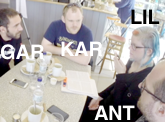
\includegraphics[width=.5\linewidth]{Graphics/3-2-Empirical-Cafe/FragmentAnimals-2}%
        \caption{Lily performs the request (\autoref{frag:empirical cafe findings answering-ii}: Do Animals Have Accents? (ii), line 44)}\label{fig:empirical cafe findings answering-ii}
    \end{figure}
    }
\end{inlinefrag}

In this second excerpt, Lily prepares to perform an utterance (line 40--42) and performs her utterance (line 42), first by moving the phone closer to her mouth with the handset held such that the microphone is in front of her lips, and then performing her utterance while there remains a gap in talk.
Following this utterance, Gary rotates his head from Antonius to Lily and responds to her question: \QF[43]{yes they do actually}.
Karl and the researcher also shift their gaze towards Lily, in the case of Karl by leaning back slightly and rotating his head, while the researcher rotates his head alone.
Through his response to Lily's question, Gary exemplifies the manner in which interactions with a \ac{VUI} are made accountable insomuch that others can observe, report upon, and respond to the device interaction accordingly---in this case, to answer the question Lily asked.
In this sense, this reveals how the preparatory action of talking to a \ac{VUI} on a personal device is made naturally accountable, and can be oriented to by co-present others as a matter occasioning further discussion.

Following this response by Gary to Lily's address to her \ac{VUI}, Lily affirms that she too had heard something\footnote{A story regarding cows with regional accents had been on the BBC News website a few days prior to this gathering.}.
In this, Lily implies that her question was guided by her being unsure (\QF{i think}, line 46), but occasioned by both the conversation and recent news events that she had read about; with Gary acknowledging he was aware of the story too (lines 46--49).
\end{revisedsubmission}



% *********************************************************************************************************************



\crpagebreak\subsubsection{Repeating a request to the VUI}\label{sec:empirical cafe findings answering repeating}
\begin{revisedsubmission}
Following this brief discussion between Lily and Gary following Lily's \ac{VUI} use, Lily has been looking at her device sporadically while talking to Gary.
She then lifts the device closer to her face again, and performs a new request to the device, which is indicated in the commencement on the next excerpt, \autoref{frag:empirical cafe findings answering-iii}.
In this next excerpt, the work of how members \textit{respond to the \ac{VUI}'s response} by repeating the request in order to accomplish their task is demonstrated. %, which, in this case, is of answering a question occasioned in conversation.

\begin{inlinefrag}
    {\fragresubmission{JR-3c: Revised fragment that is shorter}
    \begin{transcript}[51]
        \by LIL {\textbf{DO: \emph{ANIM}ALS HA\emph{V}E \emph{ACCEN}TS!}} \\
        \later  {2.4} \\
        \by LIL {°rubbish°=} \\
        \by KAR {~~~~~~~~~~~=parrots presumably do=} \\
    \end{transcript}
    \caption{Do Animals Have Accents? (iii)}\label{frag:empirical cafe findings answering-iii}
    }
\end{inlinefrag}

%This excerpt features multiple further addresses to a \ac{VUI}: first with Lily (line 51), then Lily and Karl (line 58), then the researcher (line 63), and then finally Lily (line 64).
This short excerpt features the first attempt at responding to the \ac{VUI}'s perceived failure to perform as expected, which in this case is done by repeating the request with greater volume and impetus (differing from the previous fragment in which a rephrased request was made, see \ref{sec:empirical cafe findings newinfo collab}).
As Lily does this, a gap in talk occurs (line 52) as other members look at Lily; she then quietly utters \QF[53]{rubbish}.
In and through this utterance she further accounts that the device has failed to adequately respond to the request put forward in her address to the device.
The repetition of the phrase, and increasing volume makes evident the device's failure to `hear' what is said.
Here, this demarcates a different problem with \acp{VUI}---not only do such devices have trouble responding correctly to what is said, at times they may not `hear' words at all.
\end{revisedsubmission}



% *********************************************************************************************************************



\subsubsection{Getting others to perform the request}\label{sec:empirical cafe findings answering others}
\begin{revisedsubmission}
The final excerpt from this fragment, given in \autoref{frag:empirical cafe findings answering-iv}, concludes Lily's efforts to find the answer to the question of whether animals have accents.
In this next excerpt, Lily asks Karl to help her complete the request, which she does by passing the responsibility of uttering the request to Karl by holding the device in front of Karl and questioning whether he could \QF[55, shown in \autoref{fig:empirical cafe findings answering-iv}]{ask it}.

\begin{inlinefrag}
    {\fragresubmission{JR-3c, ER-H: Revised fragment that is shorter, with labels on the image for the speakers}
    \begin{transcript}[55]
        \by LIL {~~~~~~~~~~~~~~~~~~~~~~~~~~~~~~~~~~=can you ask it?} \\
        \by     {((holds phone out in front of KAR's face))} \\
        %\im    1 {Graphics/3-2-Empirical-Cafe/FragmentAnimals-3.png}
        \by RES {((retrieves phone out of pocket))} \\
        \by KAR {\textbf{DO: ANI\emph{MALS} HAVE ACC::\emph{ENT}S!}} \\
        \later  {0.9} \\
        \by LIL {no:!} \\
        \by RES {\textit{//~sorry i'm-~//}} \\
        \by RES {((RES touches screen to stop utterance))} \\
        \by RES {\textbf{do animals have accents?}} \\
        \by LIL {\textbf{d\emph{o:} \emph{anim}als ha\emph{v}e a\emph{ccents}?}} \\
        \by RES {\textit{//~ok i've found this on the web~//} (sigh)} \\
        \by GAR {do [ they?~~]} \\
        \by LIL {~~~[ ah (.) ] it's working now!} \\
     %   \by RES {((touches top search result on device screen))} \\
    \end{transcript}
    \caption{Do Animals Have Accents? (iv)}\label{frag:empirical cafe findings answering-iv}
    \begin{figure}[bth]
        \centering
        % \renewcommand{\thesubfigure}{42}
        % \subfloat[Lily performs the request]
        %     {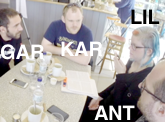
\includegraphics[width=.34\linewidth]{Graphics/3-2-Empirical-Cafe/FragmentAnimals-2}%
        %     \label{fig:empirical cafe findings answering two}} \quad
        % \renewcommand{\thesubfigure}{56}
        %\subfloat[Lily asks Karl to perform the request]
         %   {
            
\includegraphics[width=.7\linewidth]{Graphics/3-2-Empirical-Cafe/FragmentAnimals-3}
        %    \label{fig:empirical cafe findings answering three}}
        \caption{Lily asks Karl to perform the request (\autoref{frag:empirical cafe findings answering-iii}: Do Animals Have Accents? (iv), line 56)}\label{fig:empirical cafe findings answering-iv}
    \end{figure}
    }
\end{inlinefrag}

At the moment where Lily holds her device out to Karl and asks him to \QF[55]{ask it}, the researcher retrieves his phone from his pocket to perform the request (line 57).
Karl's request also fails, as revealed through Lily's next attempt (line 64), which this time yields search results, as does the researcher's (line 63).
Following the fragment, both begin to share information retrieved from webpages to the other members of the group.
This fragment is indicative of what \ac{VUI} use looks like–--that is, there are a number of grossly observable features that take place: there is ongoing selecting of speakers, repetition of requests, pauses in talk, body co-orientation and so on.

Importantly, one aspect revealed through close examination of the interaction is that once a request is performed with a \ac{VUI},  members' talk to \acp{VUI} may be sequentially followed by pauses in talk (lines 43, 52, 59), as members visibly orient their gaze towards a device as a response is computed.

% a number of practical actions are undertaken by members as they accommodate the utterance within the conversation.
% Talking to a \ac{VUI} is naturally accountable in addition to being occasioned in and through the social interaction of members in the setting.
% The accountability of action is premised on the fact that members of a setting can observe and report the action~\citep{Garfinkel1967}, and this is a feature of talk-in-interaction.
% Thus, talking to a \ac{VUI} immediately makes audible what is being undertaken to all within earshot.
% A member's device input is made directly accountable through talk, unlike interactions on touchscreens where the device user may have to provide explicit accounts to make the action accountable (as revealed in \autoref{ch:empirical pub}).
% 
% This fragment also provides interesting markers to consider what specifically follows talking to a \ac{VUI}; in particular, this transcript reveals that
The excerpts in this fragment reveal how, as a practice, talking to a \ac{VUI} in turn occasions the mutual production of silence by the co-present members as they re-orient to the use of the \ac{VUI}, and in turn focus on the device or the interlocutor.
Members do not pause their interaction or `sit in silence' however, their embodied actions of gaze and body co-orientation furnish others with how they are focusing their attention, as they turn to the device interaction.
In effect, performing a request brings about a lapse~\citep{Hoey2015} in the conversation: neither the member who was performing the request selects to talk next, nor does any other member.
\acp{VUI} function by assuming a pause-in-talk specifies the completion of a request, thus a pause by the interlocutor is necessary.
%However, as other members await a result, they do not self-select in commencing a turn.
Therefore, it is noted that the data reveals that the action of performing a request with a \ac{VUI} may prescribe a lapse in talk and the mutual production of silence.
This action is, by definition, intrinsically and demonstrably collaborative---members collectively and collaboratively socially construct silence in orientation to the utterance to the \ac{VUI}.

Furthermore, this fragment features numerous repeated requests to \acp{VUI}: Lily gets Karl to perform the request as a result of her device's repeated failure.
In the fragment, Lily uses her smartphone on multiple instances to perform the request \QF*[42, 51, 58, 63, 64]{do animals have accents?}, each time with more impetus in her voice.
With each repeated request, Lily accounts for the device's failure to appropriately respond to her initial request: either the device has mistranscribed, or it has not transcribed at all, and so another attempt is required to complete the task at hand.
Whereas in the prior fragment, members were shown to revise or \textit{rephrase} a request to get the \ac{VUI} to work, here we see another action of members to accomplish the task at hand with a \ac{VUI}: repeating the request in cases where it seems a \ac{VUI} has not `heard' the request.
Thus, a finding is that members address a problematic interaction with a \ac{VUI} through the further production of talk: \textit{they repeat their request}, and that others may assist in this completion.

% Specifically, this fragment exemplifies that members repeat requests if a request `goes wrong'; this may seem like an obvious fact but one which is worth stressing as in the corpus of observations, a total of 31 requests (25\%) were identical in lexical terms to a prior request, although lexicality is only half of the story.
% Consider in the fragment where Lily repeats her request multiple times (lines 51, 58, 64).
% Although identical in language, the production of talk differs in each one: in the first, she uses a general conversational tone; her utterance is consistent with the ongoing conversation.
% With her second performance, however, she performs the request louder and emphasises key sounds; to members within the setting, she demonstrates her frustration with the device – its failure to transcribe her words requires her to try again.
% Therefore, this analysis reveals that the failure of the device's \ac{VUI} to adequately respond to request occasions the necessity to repeat the request, possibly with greater impetus.

Finally, Lily's actions, of talking with greater impetus and volume, and then getting someone else to talk, account that for her, the perceived source of device trouble is that the device cannot transcribe her utterances because of her diction\footnote{Lily's reasoning of the trouble source is made visible as a common-sense understanding to other members of the setting, including Karl, through the second production of the request that is  produced louder and with greater impetus.}, which results in her involving Karl in the task of talking to the \ac{VUI} to complete the request.
Her practice of involving Karl in the request has the interactional outcome of recruitment to resolve the trouble at hand with the device interaction, a fundamentally collaborative mechanism of social organisation~\citep{Kendrick2016}\footnote{\citet{Kendrick2016} refer to recruitment not as single or class of social actions, but as an interactional outcome achieved through methodical practices such as requesting or offering assistance.}.
\end{revisedsubmission}



% *********************************************************************************************************************



\subsubsection{Methodical accomplishments in this fragment}\label{sec:empirical cafe findings answering methods}
\begin{revisedsubmission}
The second fragment in this chapter reveals the work of answering a question in conversation using a \ac{VUI}.
Lily \textbf{prepares to use her device} to answer the question Karl has asked, \textbf{lifting her phone to her mouth} and \textbf{addressing the \ac{VUI}} through talk.
The device ostensibly does not respond; therefore Lily \textbf{re-address the \ac{VUI} with a higher volume and impetus in her delivery but using the same question}.
The device again `fails' to respond; thus Lily \textbf{asks another co-present member, Karl, to perform the request}.
He then \textbf{addresses the \ac{VUI} with a loud speaking voice and different emphasis} compared to Lily, but with the exact same question---again there is no response from the device.
The researcher then \textbf{retrieves his phone} and \textbf{prepares his \ac{VUI} by holding the button down}.
He \textbf{addresses his \ac{VUI}} with the same question while \textbf{Lily also addresses} her \ac{VUI} again.
Both members then \textbf{verbally report that their devices have computed responses} and then go on to \textbf{discuss the findings}.
In this regard, the interactional project of using a \ac{VUI} to answer a question in conversation is completed.
\end{revisedsubmission}



% *********************************************************************************************************************



\subsection{Establishing the capability of a VUI}\label{sec:empirical cafe findings capability}
\begin{revisedsubmission}[JR-3a, JR-3c: This section is new, reconstructed from prior analysis]
The first fragment in this chapter identified how members of the setting introduce new information into a conversation by using a \ac{VUI} to retrieve the information.
The second further identified how members are able to direct specific questions raised in a conversation to a \ac{VUI}, to answer and address information deficits amongst those who are co-present.
This final fragment, which commences in \autoref{frag:empirical cafe findings capability-i} and is called \textit{Hey Siri! \ldots Call My Mother}\footnote{The complete fragment is included in \appref{app:fragments-cafe mama}.}, focuses on the researcher and Gary discussing the capability and features of the \ac{VUI} on his device, again using the \ac{VUI} to address an information deficit.
However, whereas the first two fragments identify how members are able to use a \ac{VUI} in conversation to address problems established in and through conversation, this fragment deviates from this and reveals how \ac{VUI} use may be occasioned self-referentially in order to address matters of \ac{VUI} capability\footnote{This thesis strays away from attributing a reason beyond what is naturally accountable, but the recentness with which \acp{VUI} became available at the time of this study would suggest that there is not the same level of familiarity with their capabilities as with basic smartphone interactions completed using the \ac{GUI}.}.
First, this fragment will be introduced, with the problem at hand established, and then the fragment will be unpacked as two distinct activities, in which members undertake:
\begin{enumerate}[label=(\roman*)]
    \item \nameref{sec:empirical cafe findings capability establish}, and
    \item \nameref{sec:empirical cafe findings capability testing}.
\end{enumerate}

These two activities are now unpacked in the following sections to reveal the problem case of whether the device is able to deal with a similar but non-English spelling of contact details.
\end{revisedsubmission}



% *********************************************************************************************************************



\subsubsection{Establishing the desired function}\label{sec:empirical cafe findings capability establish}
\begin{revisedsubmission}[JR-3a, JR-3c: This section is new, reconstructed from prior analysis]
The premise of the problem established through the conversation between the pair is whether the device's \ac{VUI} is capable of matching the non-English spelling of `mama' in Gary's smartphone's address book, with the discussion predicated around the focus of the study.
The conversation commences in \autoref{frag:empirical cafe findings capability-i}, in a separate floor consisting of just Gary and the researcher, who are both sitting next to each other.
The other members of the setting are conversing while the two discuss Gary's interactions with his device.

\begin{fragfloat*}
    {\fragresubmission{JR-3c, ER-H: Revised fragment that is shorter, with labels on the image for the speakers}
    \begin{transcript*}
        \by GAR {i'm curious if I say in} \\
        \by     {romanian (.) to call my mother} \\
        \later {0.7} \\
        \by GAR {it will actually find the } \\
        \by     {contact for my mother is (.)} \\
        \by     {mama in romanian (.) } \\ %if I say} \\
        \later {\ldots}[5] \\
        % \by     {call my mum will it actually} \\
        % \by     {call my mother which is in a} \\
        % \by     {contact as mama (0.7) will it} \\
        % \by     {make the connection between} \\
        % \by     {mama and mum} \\
        \by RES {cos you can also tell people} \\
        \by     {who they (.) like you can say} \\
        \by     {like} \\
        \im 1   {Graphics/3-2-Empirical-Cafe/FragmentMamma-1.png}
        \by GAR {\textbf{hey siri=}} \\
        \by RES {~~~~~~~~~=my mother is this} \\
        \by     {~~~~~~~~~~person (0.8)} \\ \vspace{3.9cm}
    \end{transcript*}
    \nopagebreak[4]
    \caption{Hey Siri! \ldots Call My Mother, part (i)}\label{frag:empirical cafe findings capability-i}
    }
\end{fragfloat*}

As this exhibit commences, Gary questions, by way of asking the researcher indirectly, whether if he asks his device to call his mother, the device will recognise the name in his contact list (the contact's name is spelt `mama' in Romanian).
The researcher responds in broken English, alluding to a feature with \acp{VUI} and smartphones that allow for pseudonyms to be allocated to contacts, although his utterance is punctuated by Gary's initial commencement of device use, using the hotword \QF[15]{hey siri}.
Without shifting his gaze from the researcher who is speaking, Gary lifts his phone and performs this phrase and then moves the device back to chest height between him and the researcher, interleaving the opening utterance of the hotword within their conversation.

Gary's initial proposition (lines 01---06) establishes that he is curious about the capability of the \ac{VUI} and its ability to function as desired.
This is followed by the researcher discussing a feature that would potentially allow Gary to request a device to call his mother, using an alternative name to the name given to the contact in his phone's address book (lines 12---14).
As such, the researcher does not directly respond to Gary's question, but makes a proposition of a technical solution to the problem at hand, by adding an English pseudonym to the contact.
\end{revisedsubmission}



% *********************************************************************************************************************



\subsubsection{Testing the functionality by addressing the VUI}\label{sec:empirical cafe findings capability testing}
\begin{revisedsubmission}
Following the continuation of the researcher's utterance regarding the pseudonym functionality (lines 16---17), Gary glances at his device and re-performs the hotword to activate his \ac{VUI}.
This next exhibit, \autoref{frag:empirical cafe findings capability-ii}, reveals how Gary tests the functionality of the \ac{VUI} with his desired capability, which allows him to demonstrate, either successfully or not, his suspicions of a limitation of the device to deal with alternative spellings of words such as \textit{mamma}.

\begin{inlinefrag}
    {\fragresubmission{JR-3c, ER-H: Revised fragment that is shorter, with labels on the image for the speakers}
    \begin{transcript*}[18]
        \by GAR {((glances down at screen))} \\
        \by     {((moves device in front of} \\
        \by     {mouth)) \textbf{hey siri}} \\
        \by GAR {((moves device to chest} \\
        \by     {height between the two))} \\
        \later  {1.0} \\
        \by RES {i'd press the button} \\
        \later  {1.2} \\
        \by GAR {((moves device in front of} \\
        \by     {mouth)) \textbf{hey siri}} \\
        \by GAR {((moves device to chest} \\
        \by     {height between the two))} \\
        \later  {2.4} \\
        \by GAR {((moves device in front of} \\
        \by     {mouth)) \textbf{call my \emph{m}other}} \\
        \im 1   {Graphics/3-2-Empirical-Cafe/FragmentMamma-2.png}
        \by     {((GAR and RES look at screen))}  \\
        \later  {5.9} \\
        \by     {\textit{// what is your mother's}} \\
        \by     {\textit{~~~name? //}} \\
        \by RES {((points towards screen)) yeah} \\
        \by     {but then} \\
        \later  {0.9} \\
        \by GAR {\textbf{my mother is mama}} \\
        \by GAR {\textit{// i can’t find anyone called}} \\
        \by     {\textit{~~~mamma //}} \\
    \end{transcript*}
    \nopagebreak[4]
    \caption{Hey Siri! \ldots Call My Mother (ii)}\label{frag:empirical cafe findings capability-ii}
    }
\end{inlinefrag}

In this excerpt, Gary glances down at his device, with the screen still dark, and so he lifts his device again and re-utters \QF*[18--20]{hey siri}.
He holds his phone in a position that the researcher can see at waist height in front of him, although this time his gaze remains on the device awaiting a result.
The researcher proffers advice based on his personal experience that he would \QF[24]{press the button}, although a moment later Gary (successfully) activates the \ac{VUI} through a further utterance of \QF[27]{hey siri} and then asks his \ac{VUI} to call his mother (line 32).
Consider the sequence of Gary's performance of this hotword: there are repeated pauses after his utterances to the \ac{VUI} (lines 15, 20, 27, 32) as Gary provides the utterance and waits for the device to respond by looking at the screen.
%Members typically pause following the completion of a hotword until the device provides a visual acknowledgement that it is `listening' (in only one instance did a member immediately follow the phrase with their request), and indeed `await' for the device to respond, suggesting a sequentiality or ordering with regarding the interaction with devices.

On completing his `test' request to the device, Gary returns to holding the device at chest level between him and his co-interlocutor, as can be seen in the image within \autoref{frag:empirical cafe findings capability-ii}, allowing both members' direct line of sight of the screen.
After nearly six seconds of both partners looking at the screen between them, the device seeks further information of the name of his mother in his address book---Gary provides this by telling the device that the contact card for his mother is \QF[40]{mama}.
This, however, does not work as the device searches for contacts named ``mamma'' and does not seemingly look for alternative spellings such as ``mama''.
The use of his \ac{VUI} is ended after this, underscoring the problem at hand that occasioned the use of the \ac{VUI} was to \textit{test and verify the functionality of the \ac{VUI}} rather than to actually call his mother.
\end{revisedsubmission}



% *********************************************************************************************************************



\subsubsection{Methodical accomplishments in this fragment}\label{sec:empirical cafe findings capability methods}
\begin{revisedsubmission}
This final fragment reveals the work of establishing the capability of a \ac{VUI} through interaction with it.
Gary establishes the capability of which he is curious, i.e. of whether the \ac{VUI} can call his mother.
He does this by questioning whether the \ac{VUI} will be able to respond to the request in conversation.
His co-interlocutor beings to respond to this question, although Gary prepares the use of his \ac{VUI} nevertheless by lifting his phone to his mouth and performing the hotword.
He does this several times as the device ostensibly does not respond to his attempts to activate the \ac{VUI}.
Once activated, he then tests the functionality of the \ac{VUI} by addressing it with the request.
The device seeks clarification of which contact details correspond to his mother, which Gary provides through a further address. The device returns a result audibly that confirms the device cannot do as Gary requested.
Although the \ac{VUI} `failed' to meet the expectations of completing the task of calling his mother---the question addressed to it---for the interactional project of establishing the capability of the \ac{VUI}, the interaction was ostensibly a `success' to the members involved.
\end{revisedsubmission}



% *********************************************************************************************************************



% \subsection{Body co-orientation}\label{sec:empirical cafe findings coorientation}
% In this fragment, the methodical practice through which members make the \ac{VUI}'s actions available to others through body co-orientation and the positioning of the device is revealed.
% The second image within the fragment in \autoref{frag:empirical cafe findings capability} shows Gary making his \ac{VUI}'s output visible to the researcher by holding his mobile phone in such a position that both parties in the conversation can orient to.
% This practice is employed by members as they make accountable the \ac{VUI}'s response through different methodical actions.
% This practice turns upon the pertinence of visibility to- and practicality of- their situated action.
% Summarily, Gary does not audibly report the failure of the device as a distinct utterance; he does this through his repetitions of the hotword and through the sharing of the visibility of the screen---he makes his actions and the outcomes of his actions available to others in and through various interactive resources\footnote{This includes his positioning of the mobile device between the pair, his gaze which is fixed on the screen, and his seating position.}.
% In undertaking work to account for his interaction, he occasions responses from the researcher by making the outcomes of the interaction with the device accountable to the setting; talking to a device occupies a turn-at-talk and recognisably is followed by further such turns.
% Therefore, in tying these findings with those from \autoref{frag:empirical cafe findings answering} together, it is noted that a \ac{VUI}'s response may not necessarily be accountable to the members of the multi-party setting, their conversational counterpart may offer this account through their actions by making the device visible, by accountably responding to the device, or through the member's production of rhetorical talk.
% Members collaboratively co-ordinate and accommodate talk to the \ac{VUI} by allowing the talk to occupy a turn in the conversation.



% *********************************************************************************************************************



%\subsection{Repetition of requests}\label{sec:empirical cafe findings repetition}
% A few seconds later her quiet utterance of \QF[53]{rubbish} suggests failure of the device to perform as expected, and this is confirmed momentarily later as she passes the responsibility of uttering the request by holding the device in front of Karl and questioning whether he could \QF[55, shown in the second photo of the figure]{ask it}.
% At this moment, the researcher retrieves his phone from his pocket to perform the request (line 57).
% The final attempt by Lily (line 64) yields search results, as does the researcher's (line 63).
% Following the fragment, both begin to share information retrieved from webpages to the other members of the group.
% This fragment is indicative of what \ac{VUI} use looks like~–--~that is, there are a number of grossly observable features that take place: there is ongoing selecting of speakers, repetition of requests, pauses in talk, body co-orientation and so on.

% The first consideration is to characterise the practice of how a member talks in turn with a \ac{VUI}.
% In the fragment, Lily uses her smartphone on multiple instances to perform the request \QF*[42, 51, 58, 63, 64]{do animals have accents?}, each time with more impetus in her voice.
% With each repeated request, Lily accounts for the device's failure to appropriately respond to her initial request: either the device has mistranscribed, or it not transcribed at all, and so another attempt is required to complete the task at hand.
% Thus, a finding is that members address a problematic interaction with a \ac{VUI} through the further production of talk: \textit{they repeat their request}.

% Specifically, this fragment exemplifies that members repeat requests if a request `goes wrong'; this may seem like an obvious fact but one which is worth stressing as in the corpus of observations, a total of 31 requests (25\%) were identical in lexical terms to a prior request, although lexicality is only half of the story.
% Consider in the fragment where Lily repeats her request multiple times (lines 51, 58, 64).
% Although identical in language, the production of talk differs in each one: in the first, she uses a general conversational tone; her utterance is consistent with the ongoing conversation.
% With her second performance, however, she performs the request louder and emphasises key sounds; to members within the setting, she demonstrates her frustration with the device – its failure to transcribe her words requires her to try again.
% Therefore, this analysis reveals that the failure of the device's \ac{VUI} to adequately respond to request occasions the necessity to repeat the request, possibly with greater impetus.

% Furthermore, members demonstrably undertake work to form collaborative action through the repetition of the request; occasioned by the failure of the \ac{VUI} to transcribe Lily's prior utterance.
% Lily's practical reasoning of the source of trouble in interaction (i.e. the device cannot transcribe her utterances because of her diction\footnote{Lily's reasoning of the trouble source is made visible as a common-sense understanding to other members of the setting, including Karl, through the second production of the request that is  produced louder and with greater impetus.}) results in her involving Karl in the task of talking to the \ac{VUI} to complete the request.
% Her practice of involving Karl in the request has the interactional outcome of recruitment to resolve the trouble at hand with the device interaction, a fundamentally collaborative mechanism of social organisation~\citep{Kendrick2016}\footnote{\citet{Kendrick2016} refer to recruitment not as single or class of social actions, but as an interactional outcome achieved through methodical practices such as requesting or offering assistance.}.



% *********************************************************************************************************************



% \subsection{Mutual production of silence}\label{sec:empirical cafe findings silence}
% Once a request is performed with a \ac{VUI}, a number of practical actions are undertaken by members as they accommodate the utterance within the conversation.
% Talking to a \ac{VUI} is naturally accountable in addition to being occasioned in and through the social interaction of members in the setting.
% The accountability of action is premised on the fact that members of a setting can observe and report the action~\citep{Garfinkel1967}, and this is a feature of talk-in-interaction.
% Thus, talking to a \ac{VUI} immediately makes audible what is being undertaken to all within earshot.
% A member's device input is made directly accountable through talk, unlike interactions on touchscreens where the device user may have to provide explicit accounts to make the action accountable (as revealed in \autoref{ch:empirical pub}).

% This fragment also provides interesting markers to consider what specifically follows talking to a \ac{VUI}; in particular, this transcript reveals that members' talk to \acp{VUI} may be sequentially followed by pauses in talk (lines 43, 52, 59), perhaps suggesting anticipation of an answer from the \ac{VUI}.
% The data shows that routinely, as a practice, talking to a \ac{VUI} in turn occasions the mutual production of silence by the co-present members as they re-orient to the accountable use of the \ac{VUI}, and in turn focus on the device or the interlocutor.
% Members do not pause their interaction or `sit in silence' however, their embodied actions of gaze and body co-orientation furnish others with how they are focusing their attention, as they turn to the device interaction.
% In effect, performing a request brings about a lapse~\citep{Hoey2015} in the conversation: neither the member who was performing the request selects to talk next, nor does any other member.
% \acp{VUI} function by assuming a pause-in-talk specifies the completion of a request, thus a pause by the interlocutor is necessary.
% However, as other members await a result, they do not self-select in commencing a turn.
% Therefore, it is noted that the data reveals that activity of performing a request with a \ac{VUI} may prescribe a lapse in talk and the mutual production of silence.
% This action is, by definition, intrinsically and demonstrably collaborative---members collectively and collaboratively socially construct silence in orientation to the utterance to the \ac{VUI}.



% % *********************************************************************************************************************



% \subsection{Accountability of the device interaction}\label{sec:empirical cafe findings accountability}
% The fragment reveals that as Lily performs her utterance to her \ac{VUI}, she, in turn, proffers a conversational topic to the floor (line 42).
% Her request is audible and accountable to all members within the multi-party conversation and is one to which any member can attend.
% Her actions were to select her \ac{VUI} to respond, but any member, as with multi-party conversation, can intervene and respond if they so choose to do so.
% The preference in multi-party conversation is for the member who was asked a question to provide an answer, but there also exists a second-order organisation for an answer to be provided by any member over the selected speaker to support the progressivity of talk~\citep{Stivers2006}.
% This organisational practice is present in this fragment as Gary answers her question with \QF[45]{yes they do actually}, choosing to provide an answer rather than wait for a response\footnote{The sequence in this fragment demonstrates the preference organisation is a matter produced through talk and not specifically that of the device interaction.
% That is, although the device interaction potentially occasions Gary to respond and certainly facilitates the ensuing interaction, it is produced as a matter of course in and through the social interaction---there is no attempt to prescribe this preference organisation to the functionality of the device or strictly as a result of interaction with devices.}.

% Gary's actions reveal that members not only orient to a \ac{VUI} or device but that members may orient and respond accordingly to the request performed.
% Moreover, although member's input to a \ac{VUI} is accountable within a multi-party conversation, a \ac{VUI} may be a muted and so not produce an audible sound within the setting.
% This is because whether it makes sounds or not is dependent upon both the manufacturer and the owner of the device (and their configuration of the device).
% In this fragment, for example, Lily's smartphone does not make an audible response to her requests, although the researcher's device does make sounds.
% Remarkably, however, the accountability of a \ac{VUI}'s response is not wholly restricted to \acp{VUI} that make audible responses or devices which are positioned so as to be visible to co-present others.
% Instead, how the interlocutor accountably attends to the performance of the request demonstrably provides a (limited) account to other members of the \ac{VUI}'s response.
% This is exemplified in Lily's repetitions of her request, occasioned by the failure of the \ac{VUI} to respond in the desired manner.

% Furthermore, this fragment reveals how members also react to a \ac{VUI}'s performance, which can be seen as Lily purports the notion of failure by muttering \QF[53]{rubbish} following her second attempt, and \QF[60]{no!} following the third.
% These utterances are not necessarily directed at any party, the group, or the device, but they make available to co-present others the failure of the device to meet her expectations.
% Therefore, although a \ac{VUI} may not audibly make its actions available to the setting, members themselves naturally account for the performance of the \ac{VUI} in and through talk, either by repeating their requests or through commenting on the device's failure with rhetoric.
% Thus, in the case of a repeated request, the member makes the device's failure to respond accordingly observable-reportable.



% *********************************************************************************************************************



% \subsection{Multimodality of feedback}\label{sec:empirical cafe findings multimodality}
% A new fragment is now introduced, given in \autoref{frag:empirical cafe findings capability}.
% In this exhibit, Gary asks his \ac{VUI} to call his mother, who is listed under the name of `mama' in his smartphone's address book.
% The conversation takes place in a separate floor consisting of just Gary and the researcher, who are both sitting next to each other.
% The other members of the setting are conversing while the two discuss Gary's interactions with his device.
% Gary ponders, by asking the researcher, whether if he asks his device to call his mother, the device will recognise the name in his contact list (the contact's name is spelt `mama' in Romanian); the action is joined as Gary attempts to accomplish this task.

% The fragment starts just after Gary picks up his phone up from the table and returns his gaze to the researcher (line 01).
% Without shifting his gaze, Gary lifts his phone and says \QF[04]{hey siri} and then moves the device back to chest height between him and the researcher.
% After a second, he glances down at his device; his smartphone's screen remains off, and so he lifts his device again and re-utters \QF[07]{hey siri}.
% He holds his phone in a position that the researcher can see, although this time his gaze remains on the device awaiting a result.
% The researcher offers implicit advice based on his personal experience (line 09), although a moment later Gary (successfully) retries \QF[11]{hey siri} and then asks his \ac{VUI} to call his mother (line 13).
% He then holds the device between the two of them again, as can be seen in the second image within \autoref{frag:empirical cafe findings capability}.
% After nearly six seconds of both partners watching the screen between them, the device seeks further information of the name of his mother in his address book — Gary provides this (line 21) although this fails as the device searches for contacts named ``mamma'' and does not seemingly look for alternative spellings such as ``mama''.
% The use of Siri is abandoned shortly after that.

% \begin{inlinefrag}
%     \begin{transcript*}
%         \by RES {cos you can also tell people} \\
%         \by     {who they (.) like you can say} \\
%         \by     {like} \\
%         \im 1   {Graphics/3-2-Empirical-Cafe/FragmentMamma-1.png}
%         \by GAR {\textbf{hey siri=}} \\
%         \by RES {~~~~~~~~~=my mother is this} \\
%         \by     {~~~~~~~~~~person (0.8)} \\
%         \by GAR {\textbf{hey siri}} \\
%         \later  {1.0} \\
%         \by RES {i'd press the button} \\
%         \later  {1.2} \\
%         \by GAR {\textbf{hey siri}} \\
%         \later  {2.4} \\
%         \by GAR {\textbf{call my \emph{m}other}\vspace*{.3cm}} \\
%         \im 1   {Graphics/3-2-Empirical-Cafe/FragmentMamma-2.png}
%         \by     {((GAR and RES watch screen))}  \\
%         \later  {5.9} \\
%         \by     {\textit{// what is your mother's}} \\
%         \by     {\textit{~~~name? //}} \\
%         \by RES {((points to screen)) yeah but} \\
%         \by     {then} \\
%         \later  {0.9} \\
%         \by GAR {\textbf{my mother is mama}} \\
%         \by GAR {\textit{// i can’t find anyone called}} \\
%         \by     {\textit{~~~mamma //}} \\
%     \end{transcript*}
%     \nopagebreak[4]
%     \caption{Hey Siri! \ldots Call My Mother}\label{frag:empirical cafe findings capability}
% \end{inlinefrag}

% In this fragment, Gary retrieves his device from the table, which in retrospect is seen as an opening to his use of the \ac{VUI}.
% He then lifts the device to his mouth but keeps the screen facing him, such that the bottom of the device is closest to his lips.
% His accountable performances of \QF[04]{hey siri} reveal his reasoning about the functionality of the device, of where the microphone is situated, and the ability of the device to `hear' one voice in a `sea' of many.
% He then holds the smartphone between him and the researcher, accordingly sustaining his device use (see \ref{sec:empirical pub findings sustaining}) and attending to the norms of social practice: he does not isolate himself or avoid interaction with the researcher, with whom he is talking.
% Additionally, he continues to use gaze and body co-orientation, and moreover, he makes visible his device screen, embedding the device and his device interaction within their conversation.
% Members may make use of a \ac{VUI}'s hotword, as Gary does in this fragment, although it is noted that of the 40 extended episodes in the corpus of data collected, only 12 featured the use of a phrase to trigger a \ac{VUI}.
% Consider the sequence of Gary's performance of this hotword: there are repeated pauses after his utterances to the \ac{VUI} (lines 08, 10, 12, 15) as Gary provides the utterance and waits for the device to respond by looking at the screen.
% Members typically pause following the completion of a hotword until the device provides a visual acknowledgement that it is `listening' (in only one instance did a member immediately follow the phrase with their request).
% These findings show that, far from shifting the modality of the interaction from visual and touch to speech, members still rely on the visual feedback from devices through glances at the screen in addition to speech as a direct consequence of the design decisions made with the \acp{VUI}.



% *********************************************************************************************************************



% \subsection{Body co-orientation}\label{sec:empirical cafe findings coorientation}
% In this fragment, the methodical practice through which members make the \ac{VUI}'s actions available to others through body co-orientation and the positioning of the device is revealed.
% The second image within the fragment in \autoref{frag:empirical cafe findings capability} shows Gary making his \ac{VUI}'s output visible to the researcher by holding his mobile phone in such a position that both parties in the conversation can orient to.
% This practice is employed by members as they make accountable the \ac{VUI}'s response through different methodical actions.
% This practice turns upon the pertinence of visibility to- and practicality of- their situated action.
% Summarily, Gary does not audibly report the failure of the device as a distinct utterance; he does this through his repetitions of the hotword and through the sharing of the visibility of the screen---he makes his actions and the outcomes of his actions available to others in and through various interactive resources\footnote{This includes his positioning of the mobile device between the pair, his gaze which is fixed on the screen, and his seating position.}.
% In undertaking work to account for his interaction, he occasions responses from the researcher by making the outcomes of the interaction with the device accountable to the setting; talking to a device occupies a turn-at-talk and recognisably is followed by further such turns.
% Therefore, in tying these findings with those from \autoref{frag:empirical cafe findings answering} together, it is noted that a \ac{VUI}'s response may not necessarily be accountable to the members of the multi-party setting, their conversational counterpart may offer this account through their actions by making the device visible, by accountably responding to the device, or through the member's production of rhetorical talk.
% Members collaboratively co-ordinate and accommodate talk to the \ac{VUI} by allowing the talk to occupy a turn in the conversation.



% *********************************************************************************************************************



% *********************************************************************************************************************


% \section{Machinery of interaction}\label{sec:empirical cafe moi}
% This work now moves from discussing the findings in terms of fragments of particular methodical and situated accomplishment, and instead reveals the resulting ``matter of interactions as products of a machinery''~\citep{Sacks1984}.

% \textbf{\textit{Performing}} a request is done by \textbf{selecting the interlocutor to perform the request from the members in the setting} through the procedurally organised practice of self-selection, as occurs when Lily chooses to ask her device whether animals have accents (\autoref{frag:empirical cafe findings answering}) or when Julia self-selects in order to determine the time of sunset (\autoref{frag:empirical cafe findings newinfo}), for example.
% Alternatively, selecting may be done through interaction with one member selecting another to perform the request in and through talk (e.g. \autoref{frag:empirical cafe findings answering}).
% Once a member is selected, the member begins by \textbf{retrieving the device and opening talk with the \ac{VUI}}.
% This is accomplished by using a hotword to enable the \ac{VUI} (e.g. \autoref{frag:empirical cafe findings capability}), or pressing the digital (e.g. \autoref{frag:empirical cafe findings answering}) or physical button (e.g. \autoref{frag:empirical cafe findings newinfo}) on the device.
% The member then undertakes the actions of \textbf{(re-)formulating and uttering the request towards the device's microphone}, with the request typically consisting of a series of keywords, an instruction (e.g. \autoref{frag:empirical cafe findings capability}), or a question (e.g. \autoref{frag:empirical cafe findings newinfo}) formed individually (e.g. \autoref{frag:empirical cafe findings capability}) or collaboratively by members through talk (e.g. \autoref{frag:empirical cafe findings newinfo}).

% \textbf{\textit{Responding}} to the request performance occurs by \textbf{mutually producing silence} in the setting as members orient to the device, the interlocutor, or the request (e.g. \autoref{frag:empirical cafe findings capability}), or by \textbf{continuing conversation amongst the other members} in accordance with standard multi-party conversational practice (e.g. \autoref{frag:empirical cafe findings answering}).
% Members undertake the routine of accounting for the \ac{VUI} by \textbf{sharing visibility of the device} (e.g. by positioning the device between them as in \autoref{frag:empirical cafe findings capability}) or by \textbf{explaining or rhetorically responding to the \ac{VUI}'s response} (e.g. exclaiming at the \ac{VUI}'s failure to hear the utterance in \autoref{frag:empirical cafe findings answering}).
% Interlocutors attend to failures by \textbf{rephrasing requests in situations where the \ac{VUI} has performed an incorrect or unexpected action} (e.g. in \autoref{frag:empirical cafe findings newinfo} when the \ac{VUI} has not understood the question posed and returns an `incorrect' answer) or by \textbf{repeating requests if the \ac{VUI} has mis–or-not-transcribed} (e.g. as occurs in \autoref{frag:empirical cafe findings answering} when the device does not hear the question posed).



% *********************************************************************************************************************



% \section{Discussion}\label{sec:empirical cafe discussion}
% The findings and the uncovered machinery will now be discussed both in terms of the existing literature and what the findings mean for the design and understanding of collocated interactions in casual-social settings when a \ac{VUI} is used.
% This work examined how a highly promoted and recently popularised interaction paradigm actually unfolds in everyday interaction.
% A setting that is common for people to socialise, relax, and use their mobile devices as part of their everyday routine was chosen.
% In this sense, the study was about exploring the use of the technology in a `real-world' (i.e. non-laboratory) setting that would always be technologically challenging for \acp{VUI}.
% Yet, studying how interactional and technological problems are accommodated in and through interaction can provide  insights for design~\citep{Norman1990}.



% % *********************************************************************************************************************



% \subsection{Repeating and rephrasing}\label{sec:empirical cafe discussion repeating}
% The collected corpus is replete with exchanges in which repetitions or rephrased requests are produced as a result of problematic interactions with the \ac{VUI} (53 out of 123 requests to a \ac{VUI}).
% The work here shows how members individually or collaboratively inspect and interpret the on-screen output of the \ac{VUI} in order to reason about and attend to the failure to complete a request.
% In the case of failures, members repeat (31 out of 123), or in some cases, rephrase their request (22 out of 123), but very few times do they abandon the request.
% Repetitions and rephrased requests happened in close succession, usually within a few seconds.
% Regarding the question how design might respond to this finding, the most obvious solution that industry probably is already working on is to explore more meaningful feedback provided by the \ac{VUI}.
% This could help the interlocutor to `find the right words', for example, by providing the grounds upon which the request failed, or by suggesting how to rephrase the request.
% Design inspiration might also be drawn from auto-completion features such as Google Instant in order to support the rephrasing of requests without the need for members to recall or reason about terms which would be more likely to result in a successful request.

% Supporting conversational repair is important, and future systems must also consider the operative language used in verbal correction.
% For example, as a human acknowledges that a \ac{VUI} has mistranscribed a word, or that they themselves have misspoken, they may say ``oh no, I meant...''.
% Further, \acp{VUI} could listen for spoken repair phrases to proactively trigger a repair sequence, in addition to the interlocutor's use of repeated or rephrased requests.
% This would reduce the effort for a human interlocutor by no longer necessitating a restart of the dialogic interaction with the \ac{VUI}.
% Additionally, the findings reveal a difficulty for \acp{VUI} to `understand'\footnote{This term is used not to suggest the machine ``understands'' in any human sense, but that it does not have the capabilities to systematically treat transcribed words as synonyms or homonyms.} synonyms and homonyms in talk.
% It is conceded, however, that it would be unrealistic to expect \acp{VUI} to demonstrate a perfect `understanding' at all times; humans are unable to achieve this themselves, and indeed as Suchman notes:

% \begin{quote}
%     \ldots there is a profound and persisting asymmetry in interaction between people and machines, due to a disparity in their relative access to the moment-by-moment contingencies that constitute the conditions of situated interaction.~\citep{Suchman2006}
% \end{quote}

% This asymmetry in the interaction\footnote{In the most reductionist of views, a machine has no access to many of the interactional resources humans methodically employ in talk. Perhaps even more problematically so, machines are incapable of parsing talk to understand simplest of paraverbal features such as intonation used in talk to provide meaning about the choice of words.} leads to a perennial debate of how a machine could demonstrate humanlike interaction without being able to detect these features.
% There are, however, mechanisms through which the existing palate of resources a machine can make use of could be more strategically used to ameliorate problematic interactions.
% Consider the function of repair in talk, and specifically the choice of words employed by humans to repair identified misunderstandings in and through ongoing interaction~\citep{Schegloff2000}.
% \acp{VUI} presently provide limited functionality for these practices; if a device has not understood a phrase, it could ask people ``could you ask your request using different words?'' or, perhaps when a word is not recognised, ``could you spell that?'', alleviating some of the identified problems.
% Such an implementation could serve as a learning opportunity for software.
% This would also provide a naturally accountable response from the \ac{VUI} that would also support multi-party conversational practices, as identified in this chapter.

% More complex speech recognition approaches have also been taken in the literature, such as an idea explored by \citet{McMillan2015} to improve the relevancy and performance of \acp{VUI}.
% In their work, they use the continuous speech stream to inform and enhance \acp{VUI} such that when they are called upon, they will have collected contextually relevant information.
% Extending this approach, the contextual relevance could be gathered from prior failed requests, as a utility to both improve accuracy in understand interlocutor's intent during successive requests, albeit at the potential expense of privacy.
% This could also be used to improve the performance of \acp{VUI} through learning various contextually relevant meanings of requests.



% % *********************************************************************************************************************



% \subsection{VUIs on portable devices as humanlike conversational partners}\label{sec:empirical cafe discussion humanlike}
% \acp{VUI}, branded as \acfp{IPA}, are generally anthropomorphised, given names (e.g. Siri), and endowed with humanistic interactional traits such as humour.
% However, their ability to support conversation is limited; they operate turn-by-turn by repeatedly cycling through simple back-and-forth input-output sequences.
% In some instances, these exchanges become expanded through additional questions posed by the \ac{VUI}, as it engages in the routine similar to ``other-initiated repair''~\citep{Schegloff1977} to seek further information from interlocutors.
% This is something that is a standard occurrence in human-to-human talk in order to repair mishearing or misinterpreting.
% Therefore, this analysis was able to explicate the humanlike orientation to conversational practice that \acp{VUI} possess.
% Members also routinely ask questions (42 out of 123 requests to \acp{VUI}) and give instructions (26 out of 123) to \acp{VUI}, suggesting that there is a perception by members to treat them as humanlike, although \citet{Luger2016} found that this was typically when in private and that in public settings people preferred the use of keywords.

% \citet{Pelikan2016} also found that people engage in `recipient design'~\citep{Sacks1974} when conversing with an artificial conversational partner as they do with human partners.
% These findings corroborate this as it was identified that members routinely reason about a response from a \ac{VUI} and attend to, either individually or collaboratively, reformulation of their request.
% These findings highlighted the mutual production of silence in talk with \acp{VUI}; these were periods of silence that become occasioned as multiple members orient to a \ac{VUI} or mobile device after a request is performed.
% This activity saw members systematically `pause' talk (but remain interactionally active through non-verbal means) as they accommodate the \ac{VUI}'s untimely response in talk, similar to the way people may orient to a question in a dinner party, for example.

% Therefore, this data reveals how the sequence of talk has some characteristics of conversation, and that talk with \acp{VUI} has the hallmarks of everyday talk between people.
% The actual performance of utterances to \acp{VUI} by members is, however, distinctly different to how one would talk to another human, even if it consists of the same or similar lexical construction.
% To illustrate this, recall \autoref{frag:empirical cafe findings answering} with the request \QF{do animals have accents?}, in which this question was repeatedly posed to a \ac{VUI}.
% In this example, Lily asks the question calmly at first, she raises her voice and employs more impetus a second time, she then asks another member to \QF[55]{ask it}, and finally, she succeeds on her fourth attempt.
% Imagine, if you will, this sequence of actions unfolding with a human counterpart instead of the \ac{VUI}: the instinctive and common-sense response would probably be that talking to someone by raising one's voice, and asking another to ``ask it'', and by another member repeating the question would be considered rude.

% Indeed, the failure of the \ac{VUI} to adequately respond to the member could also be considered rude and inattentive to the conversation.
% This development of events uncovers how talking to a \ac{VUI} is reminiscent of conversation but that the production of talk to a \ac{VUI} is fundamentally different because the recipient is not a human.
% The data reveals that members may refer to a \ac{VUI} as an `it' irrespective of the \ac{VUI}'s spoken voice being imbued with gender and this fundamentally reveals that through the veneer of humanlike interaction, members still treat a \ac{VUI} as an agent, or a machine, and not a human.
% Whether work should be done to make machines talk more like a human is contentious, with some arguing that the \textit{unformalisability} of conversation suggests efforts to create a true humanlike conversational partner are futile~\citep{Button1995a}.
% However, the purpose here has not been to discuss whether a machine could transcend from humanlike to human-realistic talk.
% Instead, the intention was to reveal the nature of talk with existing \acp{VUI} on personal devices and to highlight nuanced interactional troubles that could be addressed in future design work.
% By analytically orienting to and explicating the embodied, sequentially organised, constituent, and orderly methodical practices of how \acp{VUI} are used within a multi-party conversation, a narrative of modelling the \ac{VUI} as if it were a human interlocutor can be inferred, however, this was not the intention\footnote{This critique was raised when this work was presented at Computer-Supported Cooperative Work \& Social Computing conference 2017. The critique rests on the assumption that \acf{CA}, as an analytic practice, is \textit{only} suited to studying conversation between human partners and that it engenders and projects anthropomorphic qualities upon the actors under analysis.
% Neither is true. \ac{CA} has successfully been used both within \ac{HCI} to reveal mundane and orderly practices (e.g. \citet{Reeves2017,Norman1990}) and applied as a tool in design practice (e.g. \cite{Woodruff2002}).
% Furthermore, \ac{CA} reveals the sequential and orderly sequences of action in the setting, and with the adoption of the ethnomethodological tradition, the contingent and methodical ways in which members jointly perform action to progress the conversation and perform device interaction. The confusion that the \ac{VUI} is modelled as a human in the analysis stems from widely-used yet clumsy terminology to describe the system's actions (e.g. ``understand'' instead of compute, ``hear'' instead of transcribe) and from the humanlike qualities the systems have been imbued with by manufacturers.
% In work that uses similar practices for studying device interaction that relies on touch or gesture (e.g. \citet{Pizza2016}) such accusations are scarcely found.}.



% % *********************************************************************************************************************



% \subsection{\ac{VUI} use in multi-party conversation}\label{sec:empirical cafe discussion multiparty}
% The final discussion point is how \ac{VUI} use in multi-party conversation unfolds and the contributions of interacting through speech in a multi-party, face-to-face conversation.
% An expectation formed before going into this study was that using speech would alleviate members of the necessary accounting practices found with interaction on touchscreens, such as by explaining what a device was used for, or by sharing the screen~(see \autoref{ch:empirical pub}).
% Contravening this assumption, these findings actually show that members still provided verbal accounts for device use, particularly as they attend to failures of the \acp{VUI}.
% Furthermore, members still shared their device's screens with each other---in part because the \acp{VUI} studied rely on a touchscreen for interaction.
% The observance of members' interactions with \acp{VUI} in a casual-social setting also drew out the technical limitations of the devices, such as difficulty in the device `hearing' what was spoken to it in a bustling multi-party public setting.
% However, as technology improves these limitations will likely be eased.

% The analysis also showed how speaking to a \ac{VUI} intrinsically makes available the device interaction to all members in the setting, thus providing an opportunity for any member to engage with the device interaction and the interlocutor.
% This natural accountability has the effect of \textit{democratising the device use} by allowing any member to engage without invitation, and to intervene or collaborate with the unfolding device interaction.
% Moreover, talking to a \ac{VUI} provides a mechanism through which all within the setting can interpret and reason about not only the actions of the member who performed the request but also to reason about the request.
% In turn, each member can display practical reasoning in situations where a request failed, essentially transforming a single-person interaction with a mobile device into collaborative multi-person interaction.
% Existing research on mobile device use in collocated settings has long explored ways of supporting collaboration (e.g. \citet{Lucero2010d}), and the findings suggest that a speech-based dialogue interface could be a viable contender for this practice.



% % *********************************************************************************************************************



\section{Chapter summary}\label{sec:empirical cafe summary}
\begin{revisedsubmission}[JR-3a, JR-3c: This section has been revised in accordance with the new findings section]
%The discussion of the findings raised the question that by switching the primary mode of interaction from typing to speech, how would this interaction, and in particular, these accounting practices change?
%
%Talk to \acp{VUI} was naturally accountable because of the nature of interaction, and this led to numerous remarkable actions unfolding.
This study differs from the first study of mobile device use in \autoref{ch:empirical pub} by prescribing that members adopt a preference for using the \ac{VUI} on their device instead of interacting using the touchscreen.
The analysis of the video-recorded interactions, however, were, for the most part, identical in practice.
The first study identified how members used their device to respond to problems arising in conversation, such as to introduce new information to the conversation (see \ref{sec:empirical pub findings newinfo}) or to make jokes (see \ref{sec:empirical pub findings joke}).
Furthermore, although it may be argued the use of \acp{VUI} was `not natural', as studied, it becomes a moot argument to consider---the work in this chapter, and indeed this thesis is concerned with \textit{naturally occurring interaction around the device use}, i.e. of how members bring the device into conversation, how others orient (or not) to this, how they attend to the device through interaction, and so on.
During the studies, participants were not guided or scripted in how to `deal' with device interaction as individuals or as a group.
Therefore, were this to be a study of \textit{whether} or \textit{why} such voice-based personal device interactions occur, this would certainly be a legitimate limitation.
However as this thesis concerns itself with \textit{how} such device use is interleaved and oriented to in conversation, there is no such limitation to consider.

To summarise the findings, by pivoting to an exploration of how friends socialised around the use of the \acp{VUI} on their personal devices in a casual-social setting, this chapter revealed how they used the features to introduce new information (see \ref{sec:empirical cafe findings newinfo}) or answer questions raised in conversation (see \ref{sec:empirical cafe findings answering}).
Furthermore, however, an apparent unawareness of capabilities of \acp{VUI} was also shown to, in-part, occasion the use of the \ac{VUI} to explore and test its capabilities (see \ref{sec:empirical cafe findings capability}). 

Moreover, as with touchscreen-based device use, these activities were often accomplished while interleaving the use of the \ac{VUI} with conversation---by performing requests to the device within the conversation, by members in conversation orienting to the device through gaze and production of silence, and by collaboratively dealing with troubles that arise as a result of technical problems with the \ac{VUI}.
What becomes evident, as each successive fragment is unpacked, is that the members make the use of \acp{VUI} naturally accountable as part of the ongoing conversation in the setting, in and through the use of the device.
Additionally, the hearable request to the \ac{VUI} occasioned other co-present members' engagement with the \ac{VUI} user as a result of establishing them accounting for device use in interaction.
In contrast with touchscreen-based use, technical troubles with the \acp{VUI} were made accountable in the setting as a result the work of device users' actions, and co-present others responded to these troubles.
In this sense, using a \ac{VUI} was shown to facilitate other members attempting to complete the task on another member's behalf when technical trouble arose (see \ref{sec:empirical cafe findings answering}) or proffer suggestions on addressing technical challenges (see \ref{sec:empirical cafe findings capability}).

In conclusion, as per \autoref{ch:empirical pub}, the use of devices in the casual-social setting was occasioned in and through conversation and remained perspicuous to the members.
Additionally, \ac{VUI} use was not oriented to as problematic when occasioned, with this again being easily attributed to the very nature of the setting and purpose of the gathering (i.e. an \textit{observational study} of friends socialising).
However, in contrast to the prior study of device use, the \acp{VUI} on the smartphones were addressed as a topic in-of-itself during observations, with these conversations leading to users to explore the functionality of such systems, revealing challenges that remain at the time of study in relation to users' understandings of the capability of \acp{VUI}.


% As a request is being performed, members collaboratively pause talk for a few seconds following the request.
% In other words, members sit and wait following a request for an answer.
% Performing a request immediately embeds the device interaction in talk and can occasion further discussion relating to the request, if members so choose.
% Furthermore, the findings show that interacting with the device through speech `\textit{democratises}' the device interaction as it proffers the request as a conversational topic, and allows for any co-present member to self-select involvement in the occasioned conversation.
% When a request is produced, members may discuss the request, or the actions of the \ac{VUI} following the request.
% Additionally, they may remark, orient to, and reflect upon the resulting outcome of the interaction with the device.
% If the request failed, members may make suggestions to the device owner or choose to perform the request themselves on a personal device.
% Alternatively, the device owner may choose to perform a further request themselves, or ask another member to do so.

% Finally, although the primary mode of interaction was that of speech, members routinely make use of interactional resources such as gaze, sharing of the screen with others, and so on.
% \acp{VUI} on mobile devices do also include a visual display of the request transcription and results---members use this as part of their individual and collaborative practical reasoning and practical action in attendance to problematic outcomes.
% The effect of this is that although the \acp{VUI} are pitched as being `conversational partners', they are little more than a voice-based interface to existing functionality on the device and interacting with them defaults to touch-based interactions when the interlocutor has difficulty.
\end{revisedsubmission}

%Fortuitously, as the study in this chapter was proposed, although available for some time, \acp{VUI} on mobile devices became common place.



% *********************************************************************************************************************



\subsection{Methodical accomplishments}\label{sec:empirical cafe summary methods}
\begin{revisedsubmission}
This chapter has revealed the methodical accomplishments of using a \ac{VUI} within a multi-party conversation.
\ac{VUI} use was occasioned in talk to introduce new information into the conversation, to answer questions in talk, and to establish and test the capability of the \ac{VUI} itself.
Practically, this was done by ostensibly selecting to use ones own device, or asking another person to use the \ac{VUI}.
The device user then prepared the \ac{VUI} by pressing a button or using the hotword as an initial address to the device.
The \ac{VUI} was addressed in talk through the utterance of a request. If no response was computed by the device, the user reattempted their addressed request with a different impetus and volume.
Members would practically reason about the response from the \ac{VUI}, and if it was not `correct' would re-address the \ac{VUI} with a rephrased request.
Once the purpose of the \ac{VUI} was completed, members would either use their portable device as a normal touch screen or cease the use of the device.
\end{revisedsubmission}



% *********************************************************************************************************************



\subsection{Outlook}\label{sec:empirical cafe summary outlook}
\iresubmission[JR-2a, VV-2: The focus of this thesis is on the use of the three technologies.]{A number of `smartspeakers' were released by major technology companies and became commercially available in the UK during the analysis of this study}.
\iresubmission*[JR-2b: Specify why the technologies are suited to the home]{These devices, which require mains electricity and thus are stationary shared devices rather than portable personal devices, only support interaction through voice and do not have a touchscreen.}
The \ac{VUI} in these devices responds to questions, and can `talk back' to the user, and can also complete basic tasks such as timers, newsflashes, and music playback, as well as connecting to the Internet of Things devices.
The next chapter, \autoref{ch:empirical home}, will explore how interaction unfolds \textit{in vivo} around the use these of voice-only devices that are communal rather than personal in nature, revealing the details of how family talk around such a device ensues.
%This is especially of interest during the resolution of problematic interactions that have been shown to rely upon the screen in this chapter.



% *********************************************************************************************************************
